 \documentclass[11.5pt]{article}
\usepackage[table]{xcolor}
\definecolor{lightgray}{gray}{0.9}
\usepackage{multirow} 
\usepackage{lscape}
\usepackage{filecontents}
\usepackage[left=2.5cm,top=2.5cm,right=2.5cm,bottom=2.5cm]{geometry}
\usepackage{amsmath}
\usepackage{array}
\usepackage{caption}
\usepackage{longtable}
\usepackage{placeins}
\usepackage{graphicx}
\usepackage{subcaption}
\usepackage{setspace}
%\usepackage[active,tightpage]{preview}
\usepackage{natbib}
\bibpunct{(}{)}{,}{a}{}{;} 
\usepackage{url}
\usepackage{nth}	
\usepackage{authblk}
\usepackage{listings}
% for the d in integrals
\newcommand{\dd}{\; \mathrm{d}}
\newcommand{\tc}{\quad\quad\text{,}}
\newcommand{\tp}{\quad\quad\text{.}}
\bibliographystyle{apalike}

\title{Inequalities and deterioration in average lifespan among adults in Mexico, 1990-2015:A cross-sectional demographic cause-of-death analysis}

%\author{[authors redacted]}
\author[1]{Jos\'e Manuel Aburto}
\author[2]{Tim Riffe}
\author[3]{Vladimir Canudas-Romo}
\affil[1]{University of Southern Denmark}
\affil[2]{Max Planck Institute for Demographic Research}
\affil[3]{School of Demography, Australian National University}


\begin{document}
\newcommand{\vect}[1]{\boldsymbol{#1}}

\maketitle

\abstract
\textbf{Objective}: To quantify the effect of medically-amenable conditions, diabetes, ischemic heart diseases, lung cancer, cirrhosis, suicides, homicides and road-traffic accidents on longevity in Mexico during 1990-2015.\\

\textbf{Design}: Retrospective cross-sectional demographic analysis using aggregated data.\\

\textbf{Setting}: Vital statistics from the Mexican civil registration system.\\

\textbf{Participants}: Aggregated national data (from 91.2 million people in 1995 to 119.9 in 2015) grouped in 64 populations (32 Mexican-states [including Mexico City] by sex) with cause-of-death data.\\

\textbf{Main outcome measures}: Cause-specific contributions to the gap in life expectancy in three age groups (0-14, 15-49 and 50-84) with a low-mortality.\\

\textbf{Results}: The population below age 15 shows improvements in survival. Average survival below 15 over states was 14.82 (95\% confidence interval, 14.76 to 14.88) and 14.78 years (14.70 to 14.86) in 2015, for females and males respectively. However, the adult population aged 15 to 49 shows deterioration among males after 2006 in almost every state due to an increasing homicides and a slow recovery thereafter. Out of 35 potential years, females and males live on average 34.57 (34.48 to 34.67) and 33.80 (33.34 to 34.27), respectively. Adults aged 50 to 84 show an unexpected decrease in the low mortality benchmark, indicating nationwide deterioration in both females and males with average survival of 28.59 (27.43 to 29.75) and 26.52 (25.33 to 27.73) out of 35, respectively. State gaps from the benchmark were mainly caused by ischemic heart diseases, diabetes, cirrhosis and homicides. We find large health disparities between states, particularly for the adult population after 2005.\\

\textbf{Conclusions}: Mexico has succeeded in reducing mortality and between-state inequalities in children. However, the adult population is becoming vulnerable as it has not been able to reduce the burden of conditions amenable to health services and violence. This has led to large health disparities between Mexican states in the last 25 years.

\newpage

\section*{Supplemental material}
Appendix Table 1. Definitions of cause-of-death categories using the \nth{9} and \nth{10} revision of the International Classification of Diseases.\\

{\renewcommand{\baselinestretch}{1}\selectfont

%\begin{longtable}{p{8cm}p{4cm}p{4cm}ccc}
%\hline
%\textbf{Category} & \textbf{ICD-10} & \textbf{ICD-9}\\
%\hline
%\endfirsthead
%\multicolumn{3}{c}%
%{\tablename\ \thetable\ -- \textit{Continue}} \\
%\hline
%\textbf{Category} & \textbf{ICD-10} & \textbf{ICD-9}\\
%\hline
%\endhead
%\hline \multicolumn{3}{r}{\textit{Continues}} \\
%\endfoot
%\hline
%\endlastfoot
%\multicolumn{3}{l}{\bf I. Amenable to medical service}  \\
% I.A. AM-Infectious \& respiratory diseases : intestinal infections, tuberculosis, zoonotic bacterial diseases, other bacterial diseases, septicemia, poliomyelitis, measles, rubella, infectious hepatitis, ornithosis, rickettsioses/ arthropod-borne, syphilis (all forms), yaws, respiratory diseases, influenza \& pneumonia, chronic lower respiratory diseases & A00-A09, A16-A19, B90, A20-A26, A28, A32, A33, A35, A36, A37, A40-A41, A80, B05-B06, B15-B19, A70, A68, A75, A77, A50-A64, A66, J00-J08, J20-J39, J60-J99, J09-J18, J40-J47 & 001-009, 010-018, 32, 33, 37, 137, 020-027, 38, 45, 55-56, 70, 73, 080-082, 087, 090-099, 102, 460-479, 500-519, 480-488, 490-496 \\
%           I.B. AM-Cancers: malignant neoplasm of colon, skin, breast, cervix, prostate, testis, bladder, kidney-Wilm's tumor only, eye, thyrodid carcinoma, Hodgkin’s disease, leukemia & C16,C18-C21, C43-C44, C50, C53, C61, C62, C67, C64, C69, C73, C81, C91-C95 & 153-154, 172-173, 174, 180, 185, 186, 188-189, 190, 193, 201, 204-208\\
%           I.C. AM-Circulatory: active/acute rheumatic fever, chronic rheumatic heart disease, hypertensive disease, cerebrovascular disease & I00-I02, I05-I09, I10-I13, I15, I60-I69 & 390-392, 393-398, 401-405, 430-438\\
%          I.D. AM-Birth: maternal deaths (all), congenital cardiovascular anomalies, perinatal deaths (excluding stillbirths) & O00-O99, Q20-Q28, P00-P96 & 630-676, 745-747, 760-779\\
%          I.E. AM-Other: disease of thyroid, epilepsy, peptic ulcer, appendicitis, abdominal hernia, cholelithiasis \& cholecystitis, nephritis, benign prostatic hyperplasia, misadventures to patients during surgical or medical care, cisticerchosis & E00-E07, 40-G41, K25-K27, K35-K38, K40-K46, K80-K81,  N00-N07, N17-N19, N25-N27, N40, Y60-Y69, Y83-Y84, B69 & 240-246, 345, 531-533, 540-543, 550-553, 574-575.1, 580-589, 600, E870-E876, E878-E879\\
% & \\          
% {\bf II. Diabetes}  & E10-E14 & 250 \\      
% & \\
% {\bf III. Ischemic Heart Diseases (IHD)}   & I20-I25 & 410-414, 429.2\\
% & \\           
% {\bf IV. HIV/AIDS} & B20-B24 & 279.1, 042-044\\ 
%  & \\                
%{\bf V. Lung cancer}  & C33-C34 & 162\\
%  & \\          
%{\bf VI. Cirrhosis}&  K70 & 571.1-571.3\\
% & \\          
%{\bf VII. Homicides}  & X85-Y09 & E960-E969\\     
% & \\           
% {\bf VIII. Road traffic accidents}  & V01-V99 & E810-E819 \\     
% & \\           
%{\bf IX. Suicide and self-inflicted injuries}  & U03, X60-X84, Y87.0 & E950-E959\\ 
% & \\          
%{\bf X. Residual Causes }:  HIV/AIDS; suicide and self-inflicted injuries; other cancers and other heart diseases & B20-B24, U03; X60-X84, Y87.0; C00-D48; I00-I99 if not listed above; R00-R99 & 042-044; E950-E959; 140-239; 390-459 if not listed above; 780-799
%\label{ME_Mex}
%\end{longtable}

\begin{longtable}{p{8cm}p{4cm}p{4cm}ccc}
\hline
\textbf{Category} & \textbf{ICD-10} & \textbf{ICD-9}\\
\hline
\endfirsthead
\multicolumn{3}{c}%
{\tablename\ \thetable\ -- \textit{Continue}} \\
\hline
\textbf{Category} & \textbf{ICD-10} & \textbf{ICD-9}\\
\hline
\endhead
\hline \multicolumn{3}{r}{\textit{Continues}} \\
\endfoot
\hline
\endlastfoot
\multicolumn{3}{l}{\bf I. Amenable to medical service}  \\
 I.A. AM-Infectious \& respiratory diseases : intestinal infections, tuberculosis, zoonotic bacterial diseases, other bacterial diseases, septicemia, poliomyelitis, measles, rubella, infectious hepatitis, ornithosis, rickettsioses/ arthropod-borne, syphilis (all forms), yaws, respiratory diseases, influenza \& pneumonia, chronic lower respiratory diseases & A00-A09, A16-A19, B90, A20-A26, A28, A32, A33, A35, A36, A37, A40-A41, A80, B05-B06, B15-B19, A70, A68, A75, A77, A50-A64, A66, J00-J08, J20-J39, J60-J99, J09-J18, J40-J47 & 001-009, 010-018, 32, 33, 37, 137, 020-027, 38, 45, 55-56, 70, 73, 080-082, 087, 090-099, 102, 460-479, 500-519, 480-488, 490-496 \\
           I.B. AM-Cancers: malignant neoplasm of colon, skin, breast, cervix, prostate, testis, bladder, kidney-Wilm's tumor only, eye, thyroid carcinoma, Hodgkin’s disease, leukemia & C16,C18-C21, C43-C44, C50, C53, C61, C62, C67, C64, C69, C73, C81, C91-C95 & 153-154, 172-173, 174, 180, 185, 186, 188-189, 190, 193, 201, 204-208\\
           I.C. AM-Circulatory: active/acute rheumatic fever, chronic rheumatic heart disease, hypertensive disease, cerebrovascular disease & I00-I02, I05-I09, I10-I13, I15, I60-I69 & 390-392, 393-398, 401-405, 430-438\\
          I.D. AM-Birth: maternal deaths (all), congenital cardiovascular anomalies, perinatal deaths (excluding stillbirths) & O00-O99, Q20-Q28, P00-P96 & 630-676, 745-747, 760-779\\
          I.E. AM-Other: disease of thyroid, epilepsy, peptic ulcer, appendicitis, abdominal hernia, cholelithiasis \& cholecystitis, nephritis, benign prostatic hyperplasia, misadventures to patients during surgical or medical care, cisticerchosis & E00-E07, 40-G41, K25-K27, K35-K38, K40-K46, K80-K81,  N00-N07, N17-N19, N25-N27, N40, Y60-Y69, Y83-Y84, B69 & 240-246, 345, 531-533, 540-543, 550-553, 574-575.1, 580-589, 600, E870-E876, E878-E879\\
 & \\          
 {\bf II. Diabetes}  & E10-E14 & 250 \\      
 & \\
 {\bf III. Ischemic Heart Diseases (IHD)}   & I20-I25 & 410-414, 429.2\\
 & \\                          
{\bf IV. Lung cancer}  & C33-C34 & 162\\
  & \\          
{\bf V. Cirrhosis}&  K70 & 571.1-571.3\\
 & \\          
{\bf VI. Homicides}  & X85-Y09 & E960-E969\\     
 & \\           
 {\bf VII. Road traffic accidents}  & V01-V99 & E810-E819 \\              
 & \\          
  {\bf VIII. Suicide and self-inflicted injuries}  & E950-E959 & X60-X84, Y87.0\\              
 & \\          
{\bf IX. Residual Causes }:  HIV/AIDS; other cancers and other heart diseases & B20-B24, U03; C00-D48; I00-I99 if not listed above; R00-R99 & 042-044;140-239; 390-459 if not listed above; 780-799
\label{ME_Mex}
\end{longtable}

\newpage

\subsection*{Temporary Life Expectancy}
Temporary life expectancy between ages
$x_1$ and $x_2$, for $x_1<x_2$, is defined as the average years of life lived between these ages according to a given set of mortality rates \citep{arriaga1984}. We denote this quantity as
$_{(x_2-x_1)}e_{x_1}$, and its benchmark based on minimum death rates for every age and cause of death among the Mexican states for each year as $_{(x_2-x_1)}e^{\star}_{x_1}$. Defined in
terms of the lifetable survival function, $\ell(x)$:

\begin{equation}
_{(x_2-x_1)}e_{x_1} = \frac{\int _{x_1}^{x_2} \ell(x) \dd x}{\ell(x_1)}
\end{equation}

If full survival is achieved, the life expectancy is $x_2-x_1$.  For example, if we set $x_1=0$ and $x_2=15$, and no person dies between the ages 0 and 15, on average the population lives 15 full years.

\subsection*{Decomposition method}

The decomposition method used in this paper relies on a model of demographic functions based on continuous change \citep{horiuchi2008}. Suppose $P$ (e.g. temporary life expectancy between ages 15 and 49) is a differentiable function of $n$ covariates (e.g. each age-cause specific mortality rate) denoted by the vector $\vect{A} = \left[x_1,x_2,\ldots,x_n \right]^T$. We assume that $\vect{A}$ is a differentiable function between $P_1$ and $P_2$, then the difference in $P$ between $P_1$ and $P_2$ can be expressed as follows:
\begin{equation}
\label{eq.decom}
P_2-P_1 = \sum_{i = 1}^n \int_{x_i(P_1)}^{x_i(P_2)}\frac{\partial P}{\partial x_i}dx_i=\sum_{i = 1}^nc_i ,
\end{equation}
where $c_i$ is the total change in $P$ produced by changes in the $i$-th covariate, $x_i$. The $c_i$'s in equation \eqref{eq.decom} were computed by numerical integration following the algorithm suggested by \citet{horiuchi2008}. This method has the advantage of assuming that covariates change gradually along the time dimension.


\begin{figure}
\centering
\caption{Cause-specific death counts (different $y$-scale for each cause), 1990-2010.}
\label{fig:ClassSens}
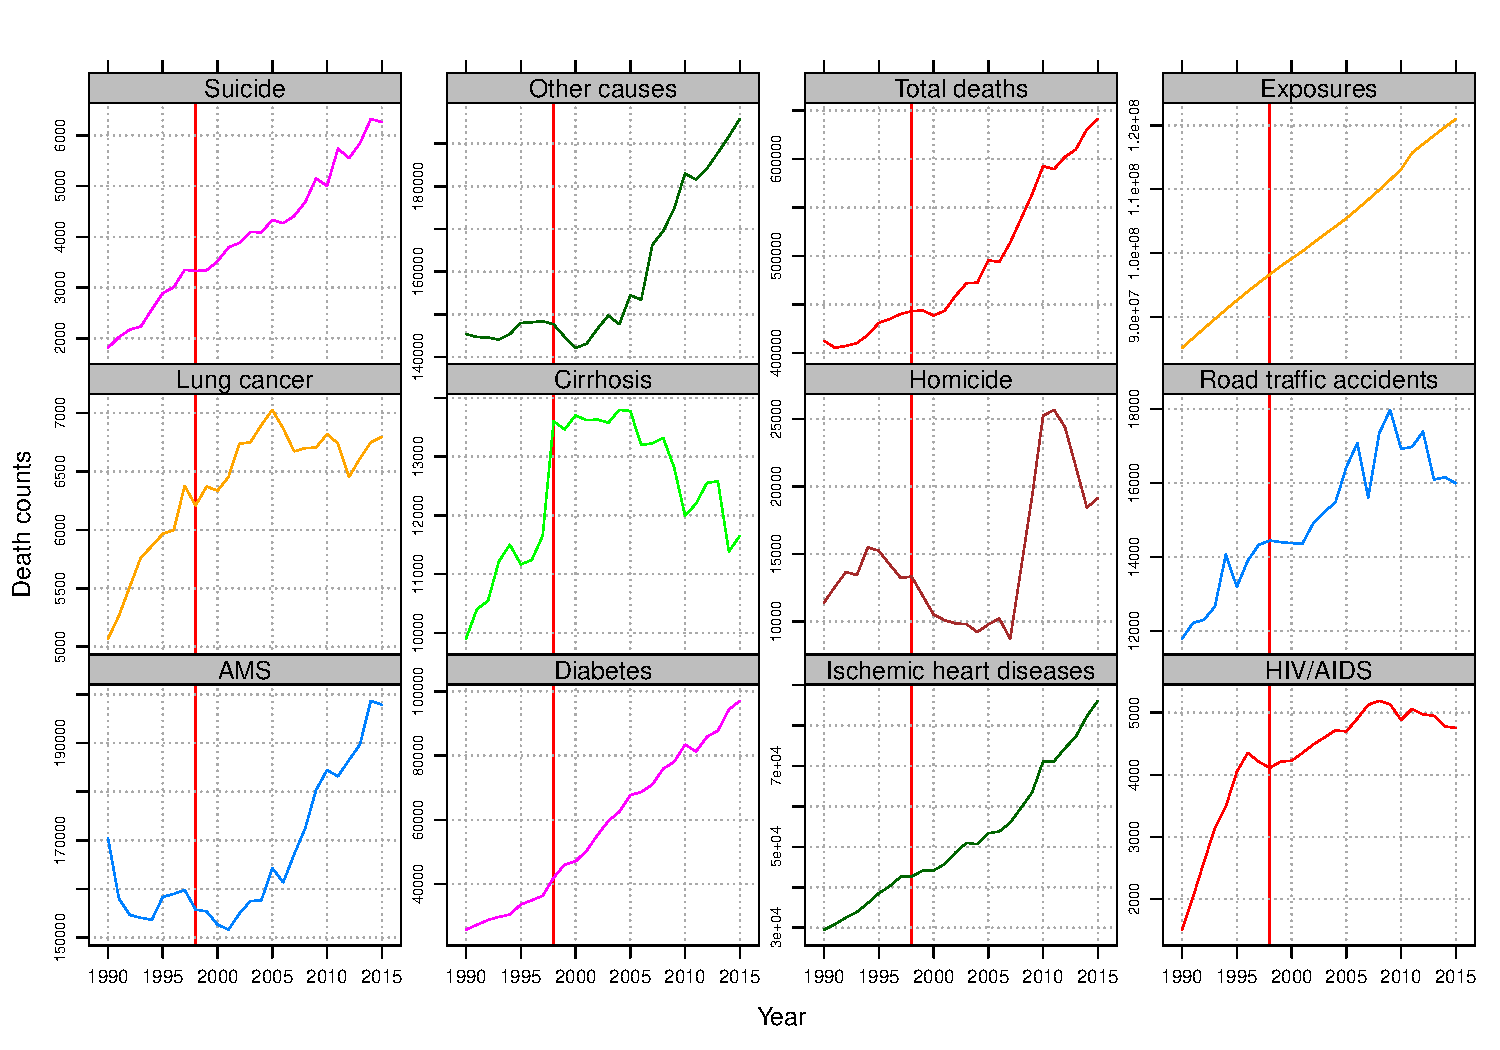
\includegraphics[scale=.65]{Figures/Sensitivity_fig.pdf}

Note: AMS ``amenable to medical service''. The red line indicates the change from ICD 9 to ICD 10. 
\end{figure}


\section*{Robustness check: 95\% CIs for male temporary life expectancies}


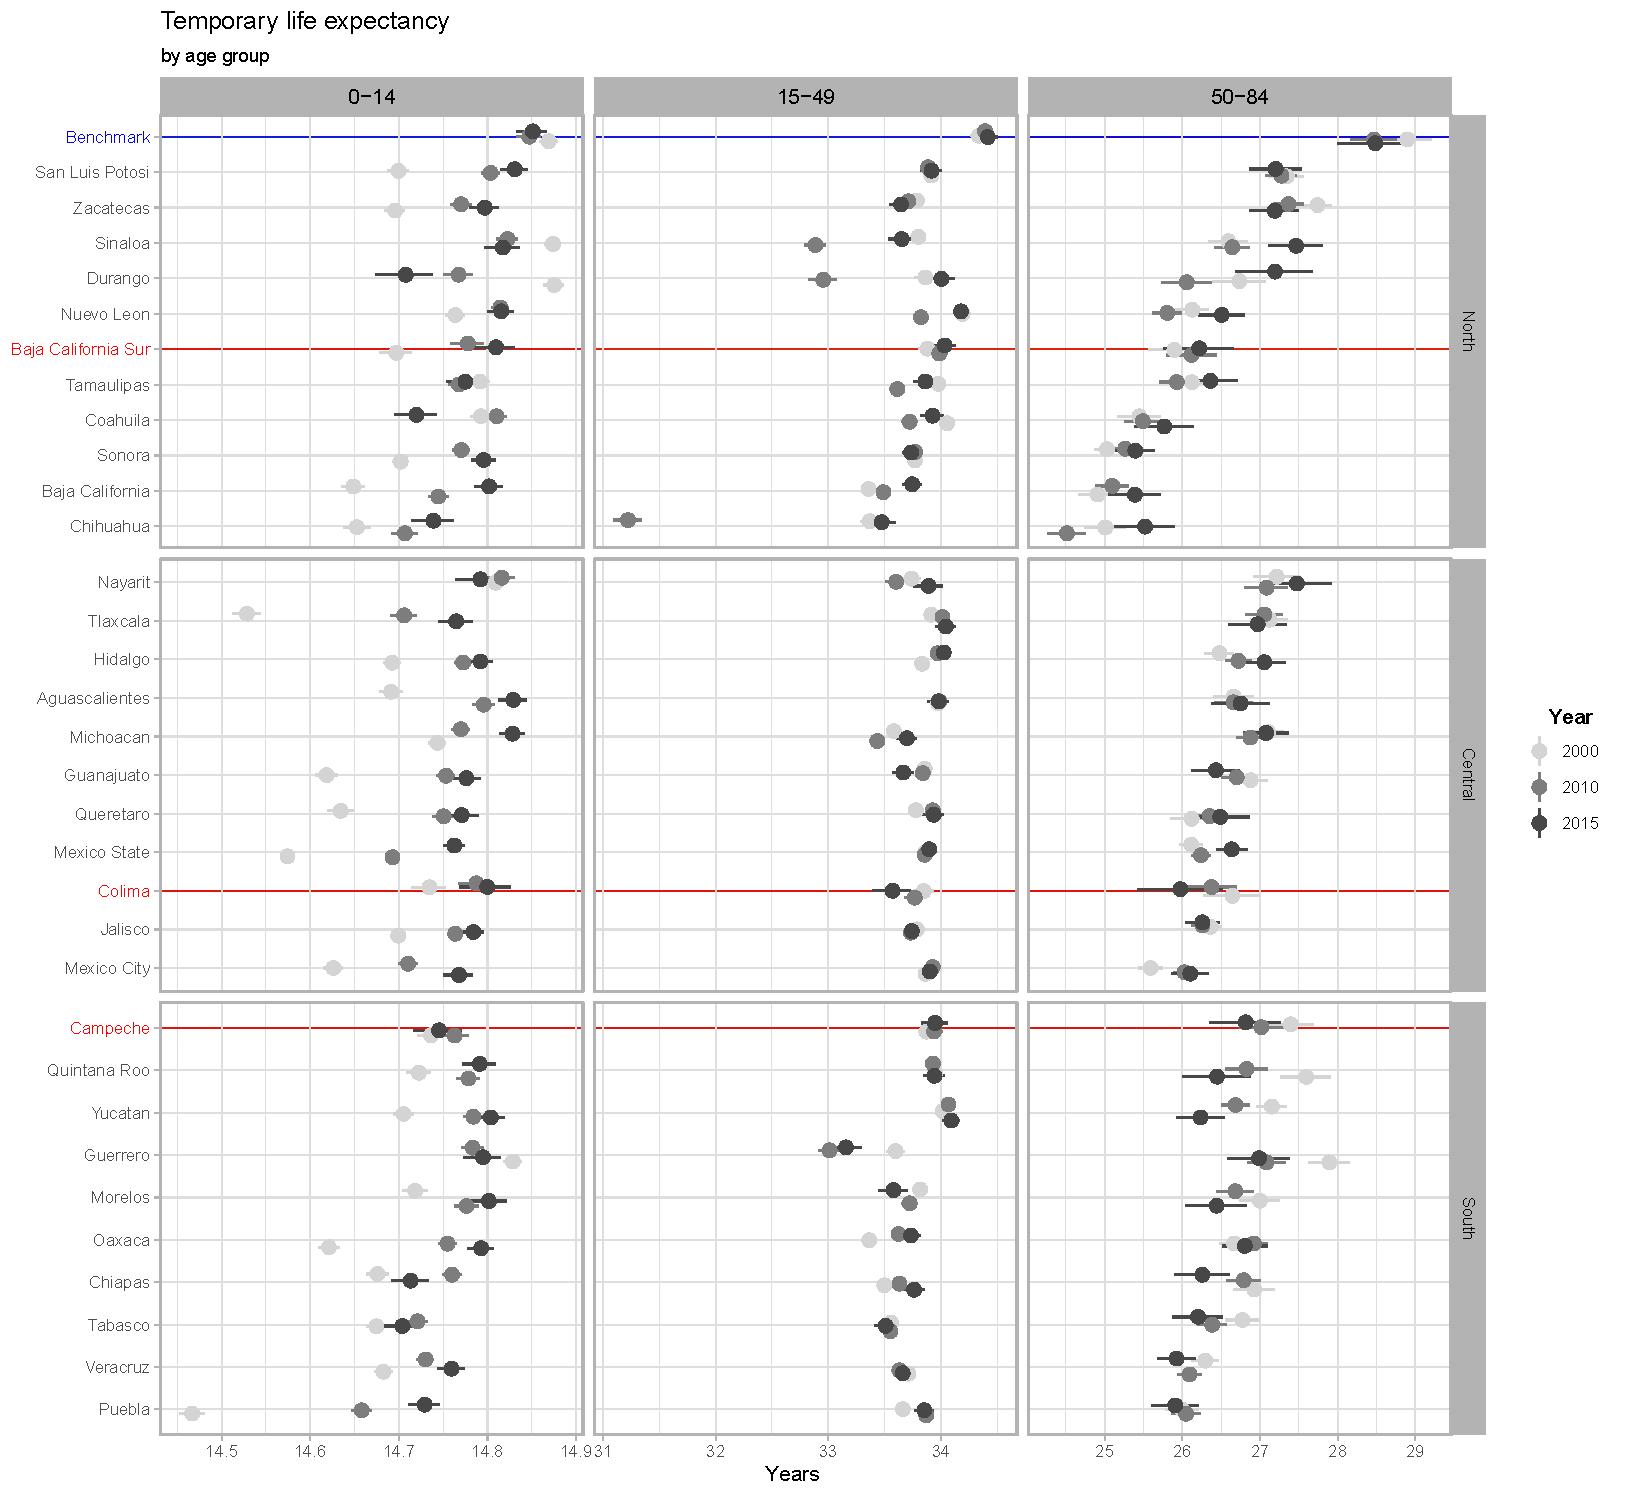
\includegraphics[scale=.65]{Figures/Temp_e0_CIs_RR_Final.pdf}
Note: States highlighted in red had less than 1 million population in 2010.



\begin{figure}[h!]
\centering
\caption{Inequality in life expectancy between states for youngest (0-14), young adults (15-49), and older adults (50-84) by sex, 1990-2015.}
\label{fig:Gini}
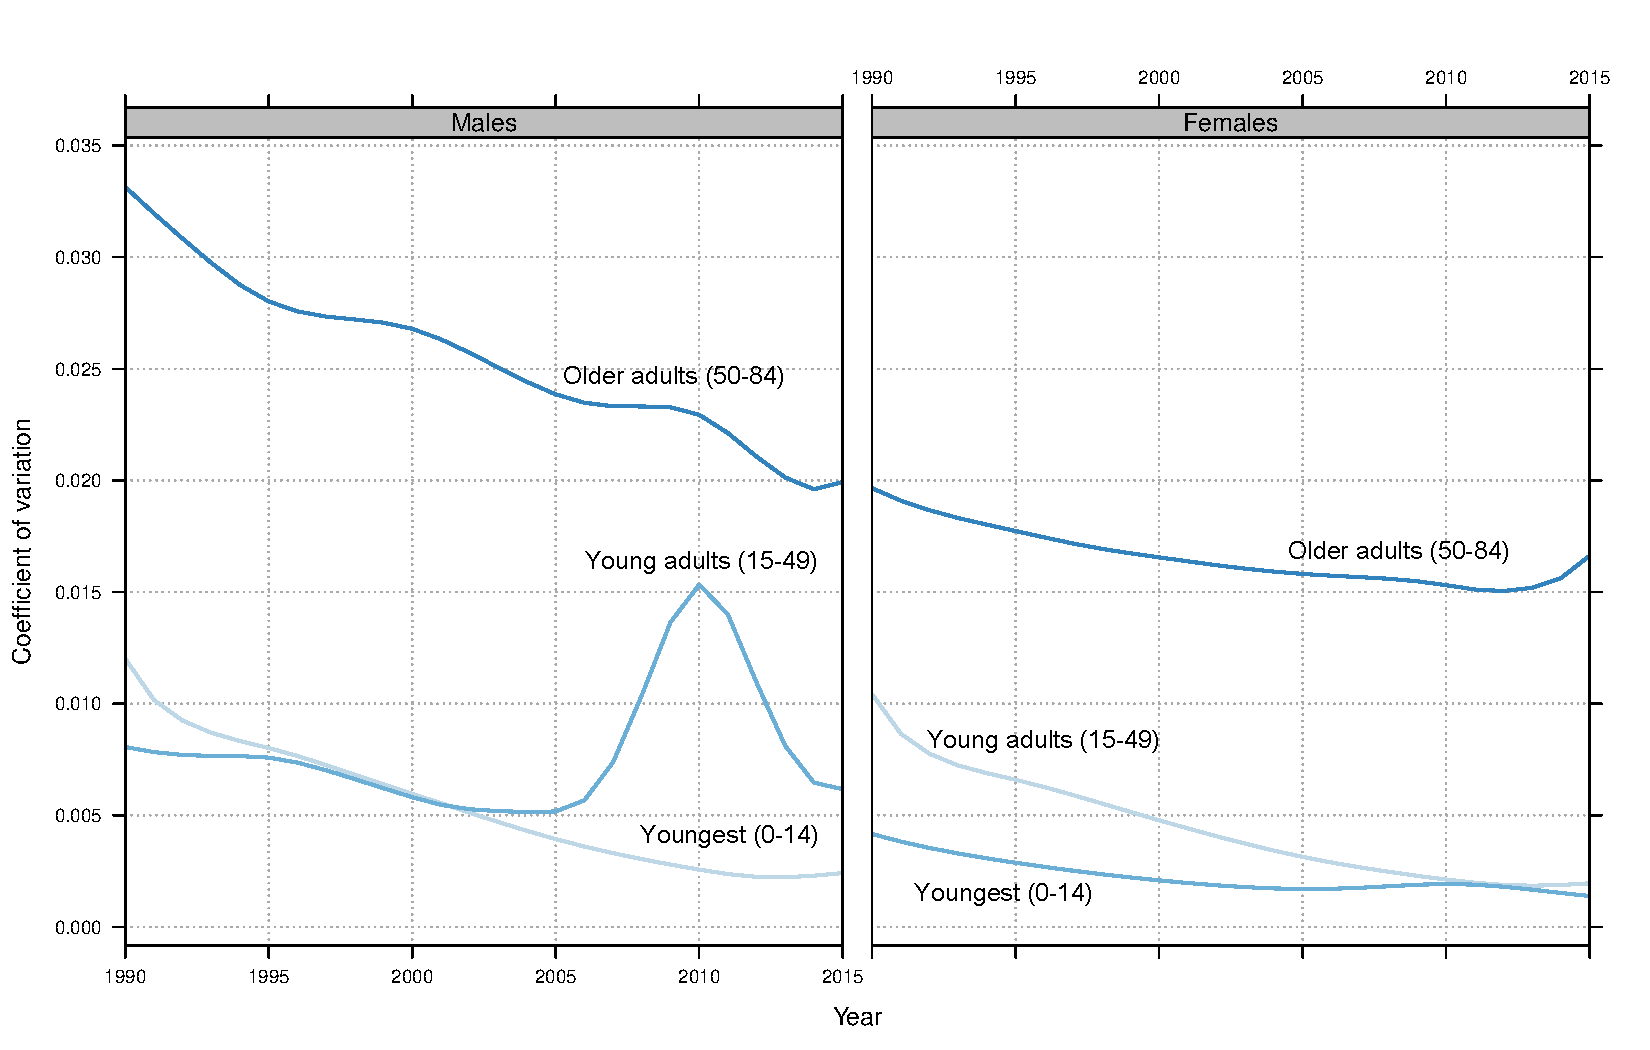
\includegraphics[scale=.45]{Figures/CVfig.pdf}
\end{figure}

\begin{figure}[h!]
\centering
\caption{State ranking for average female life expectancy 2010-15 for the youngest (0-14), young adults (15-49), and older adults (50-84).}
\label{rankFemales}
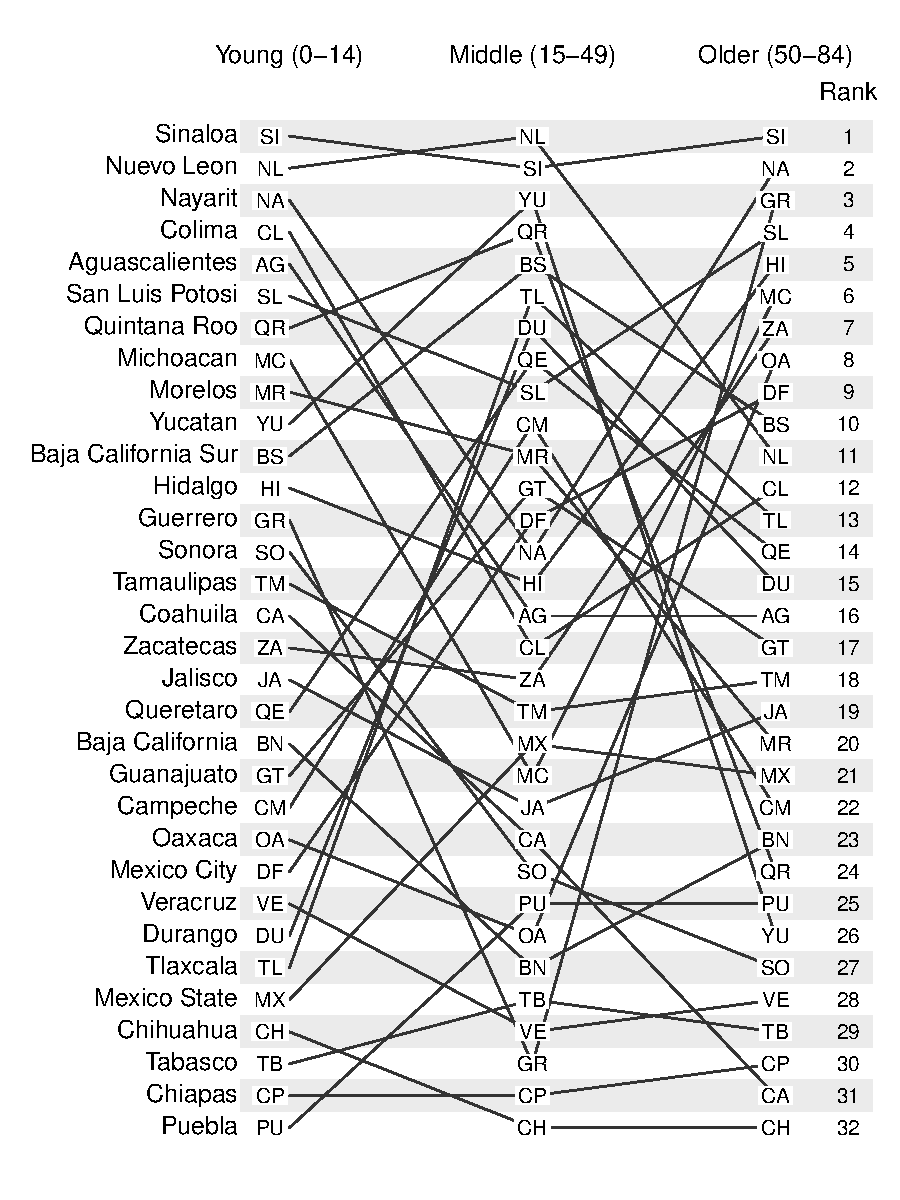
\includegraphics[scale=.50]{Figures/RankFemales.pdf}

Source: calculations based on INEGI and CONAPO files. 
\end{figure}

\begin{figure}[h!]
\centering
\caption{Cause-specific contributions to state differences from low mortality benchmark for older male adults (ages 50-84), 1990-2015. States grouped into three regions. Reproduced from manuscript Figure 4 to have color scale comparable with other Supplementary figures. In subsequent figures 5-9 the color was rescaled to make them comparable over age groups in the supplemental material, the maximum value observed was 2.6 years caused by homicides in Chihuahua in 2010.}
\label{fig:e40_74_males}
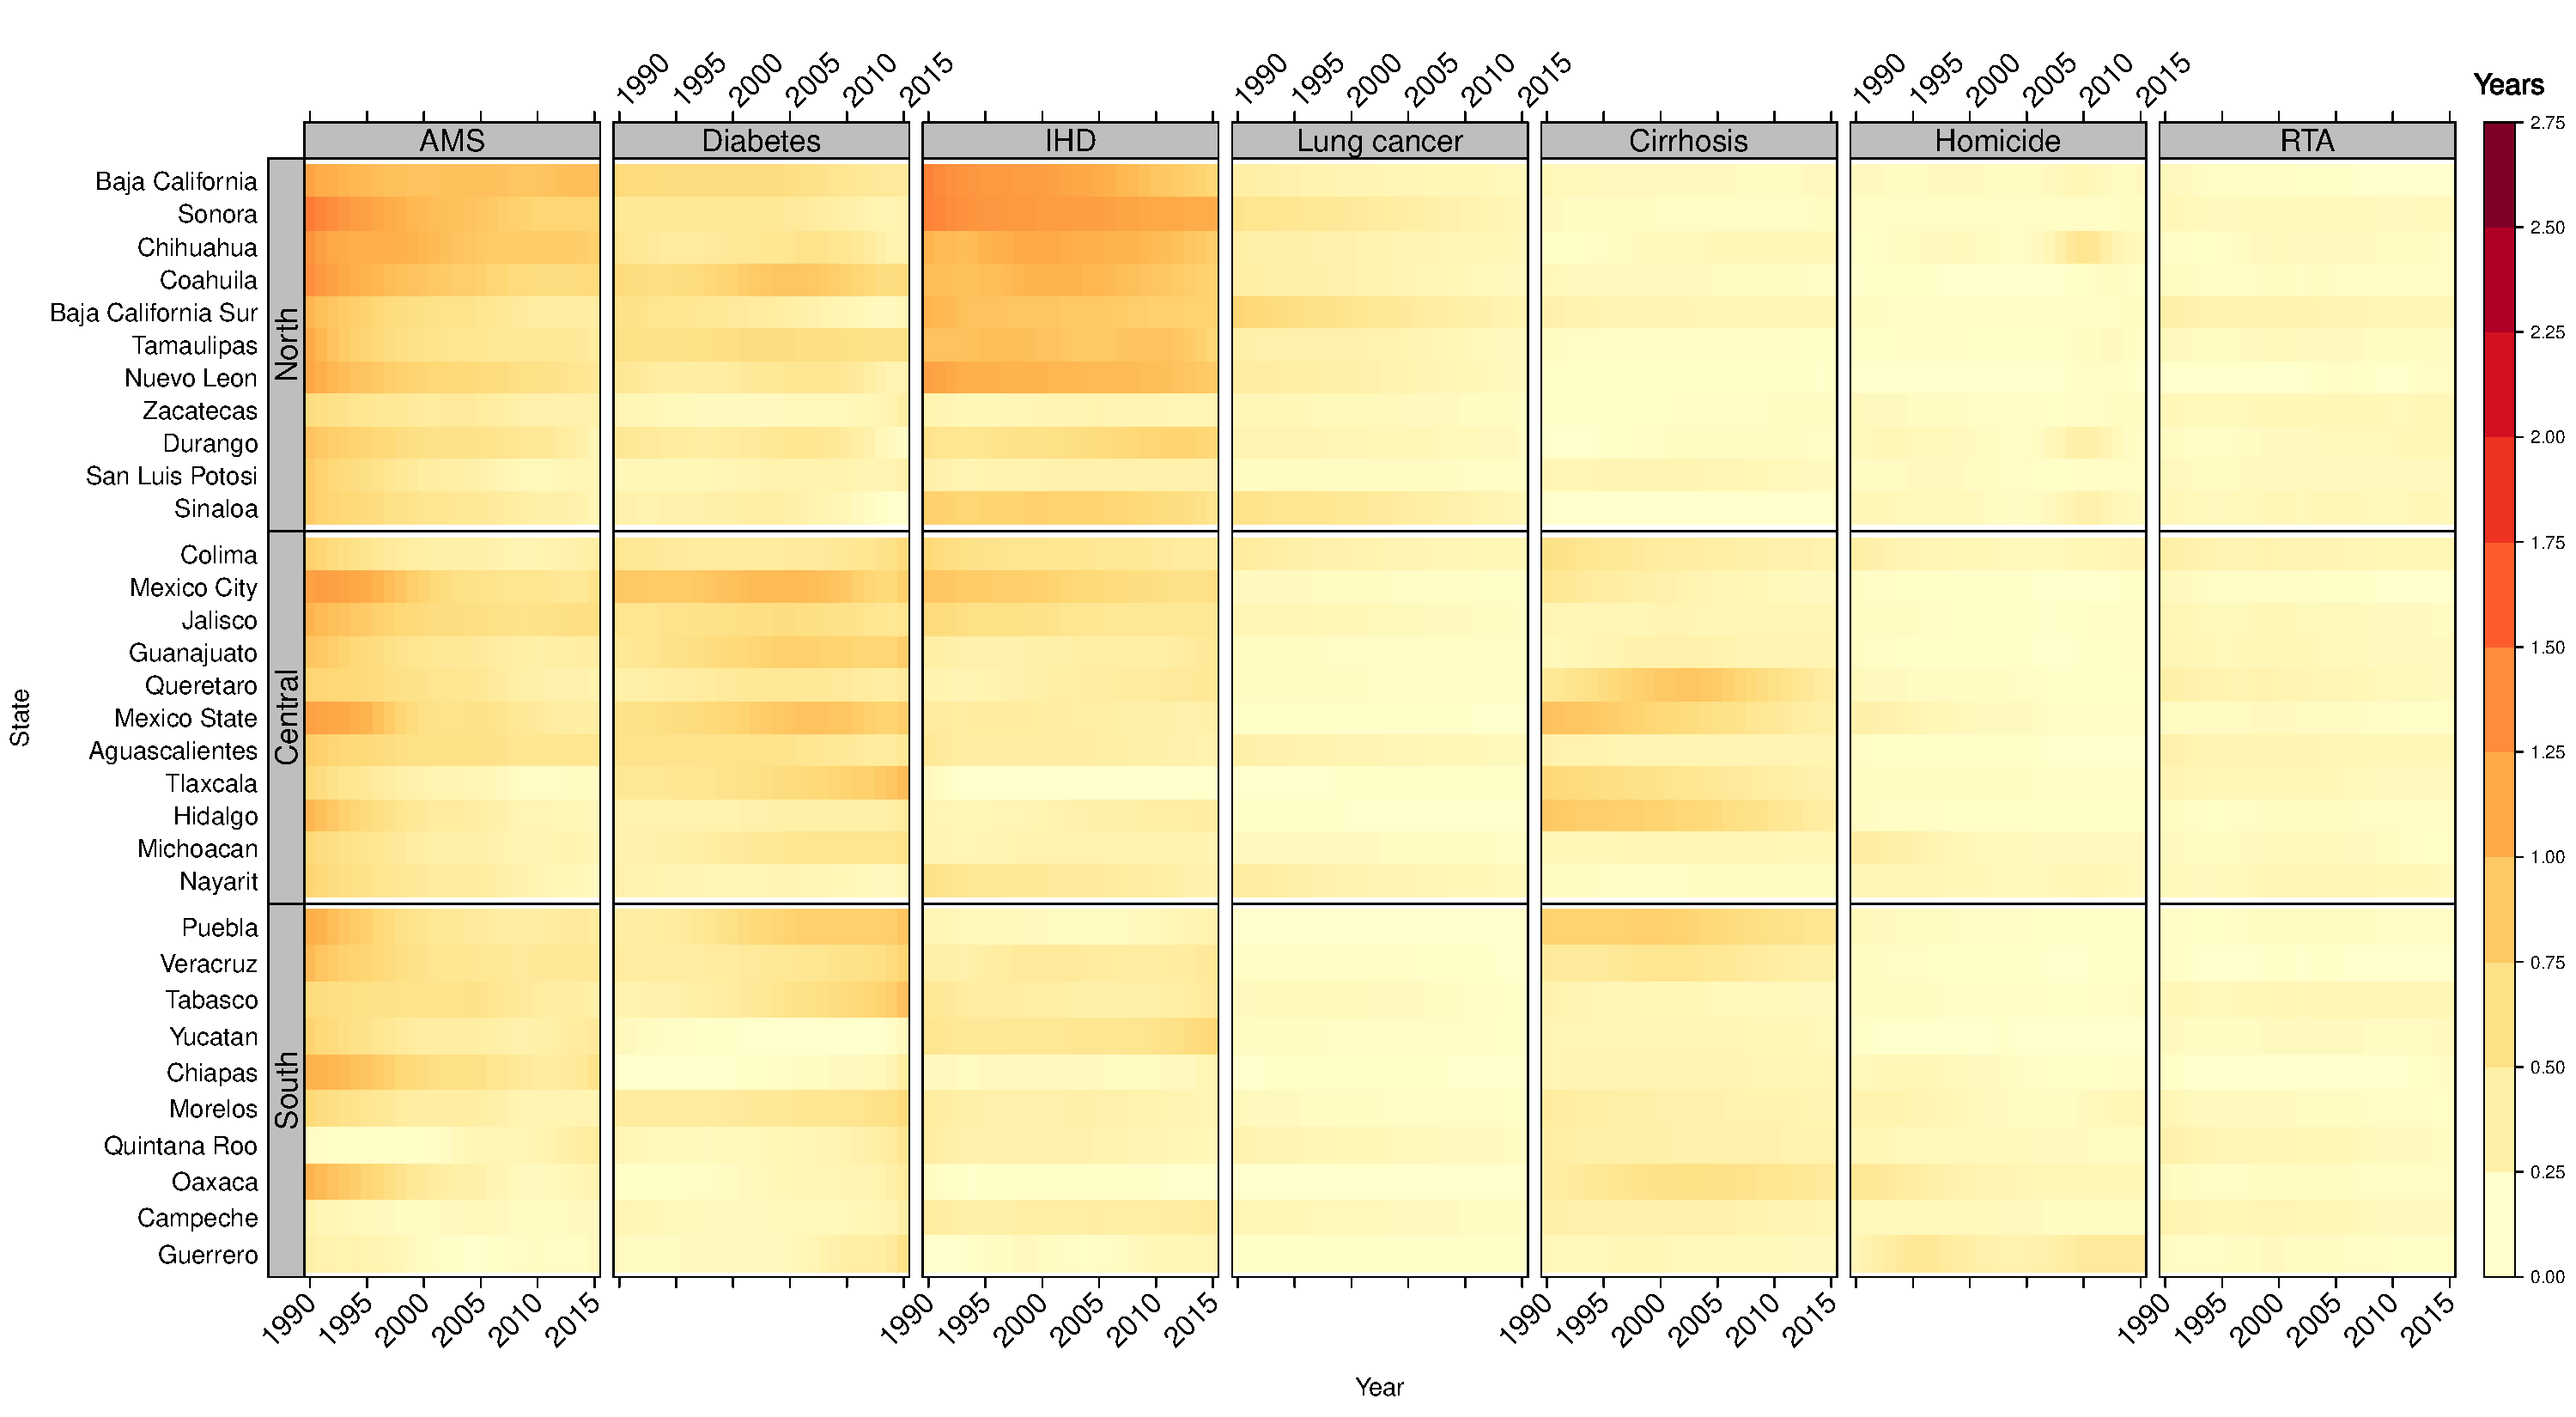
\includegraphics[scale=.30]{Figures/Adult_Male_heatmap.pdf}
Note: AMS is ``amenable to medical service'', IHD is ``isquemic heart diseases'', and RTA is ``road traffic accidents''. Source: own calculations. \end{figure}

\begin{figure}[h!]
\centering
\caption{Cause-specific contributions to state differences from low mortality benchmark for older female adults (ages 50-84), 1990-2015.}
\label{fig:e40_74_females}
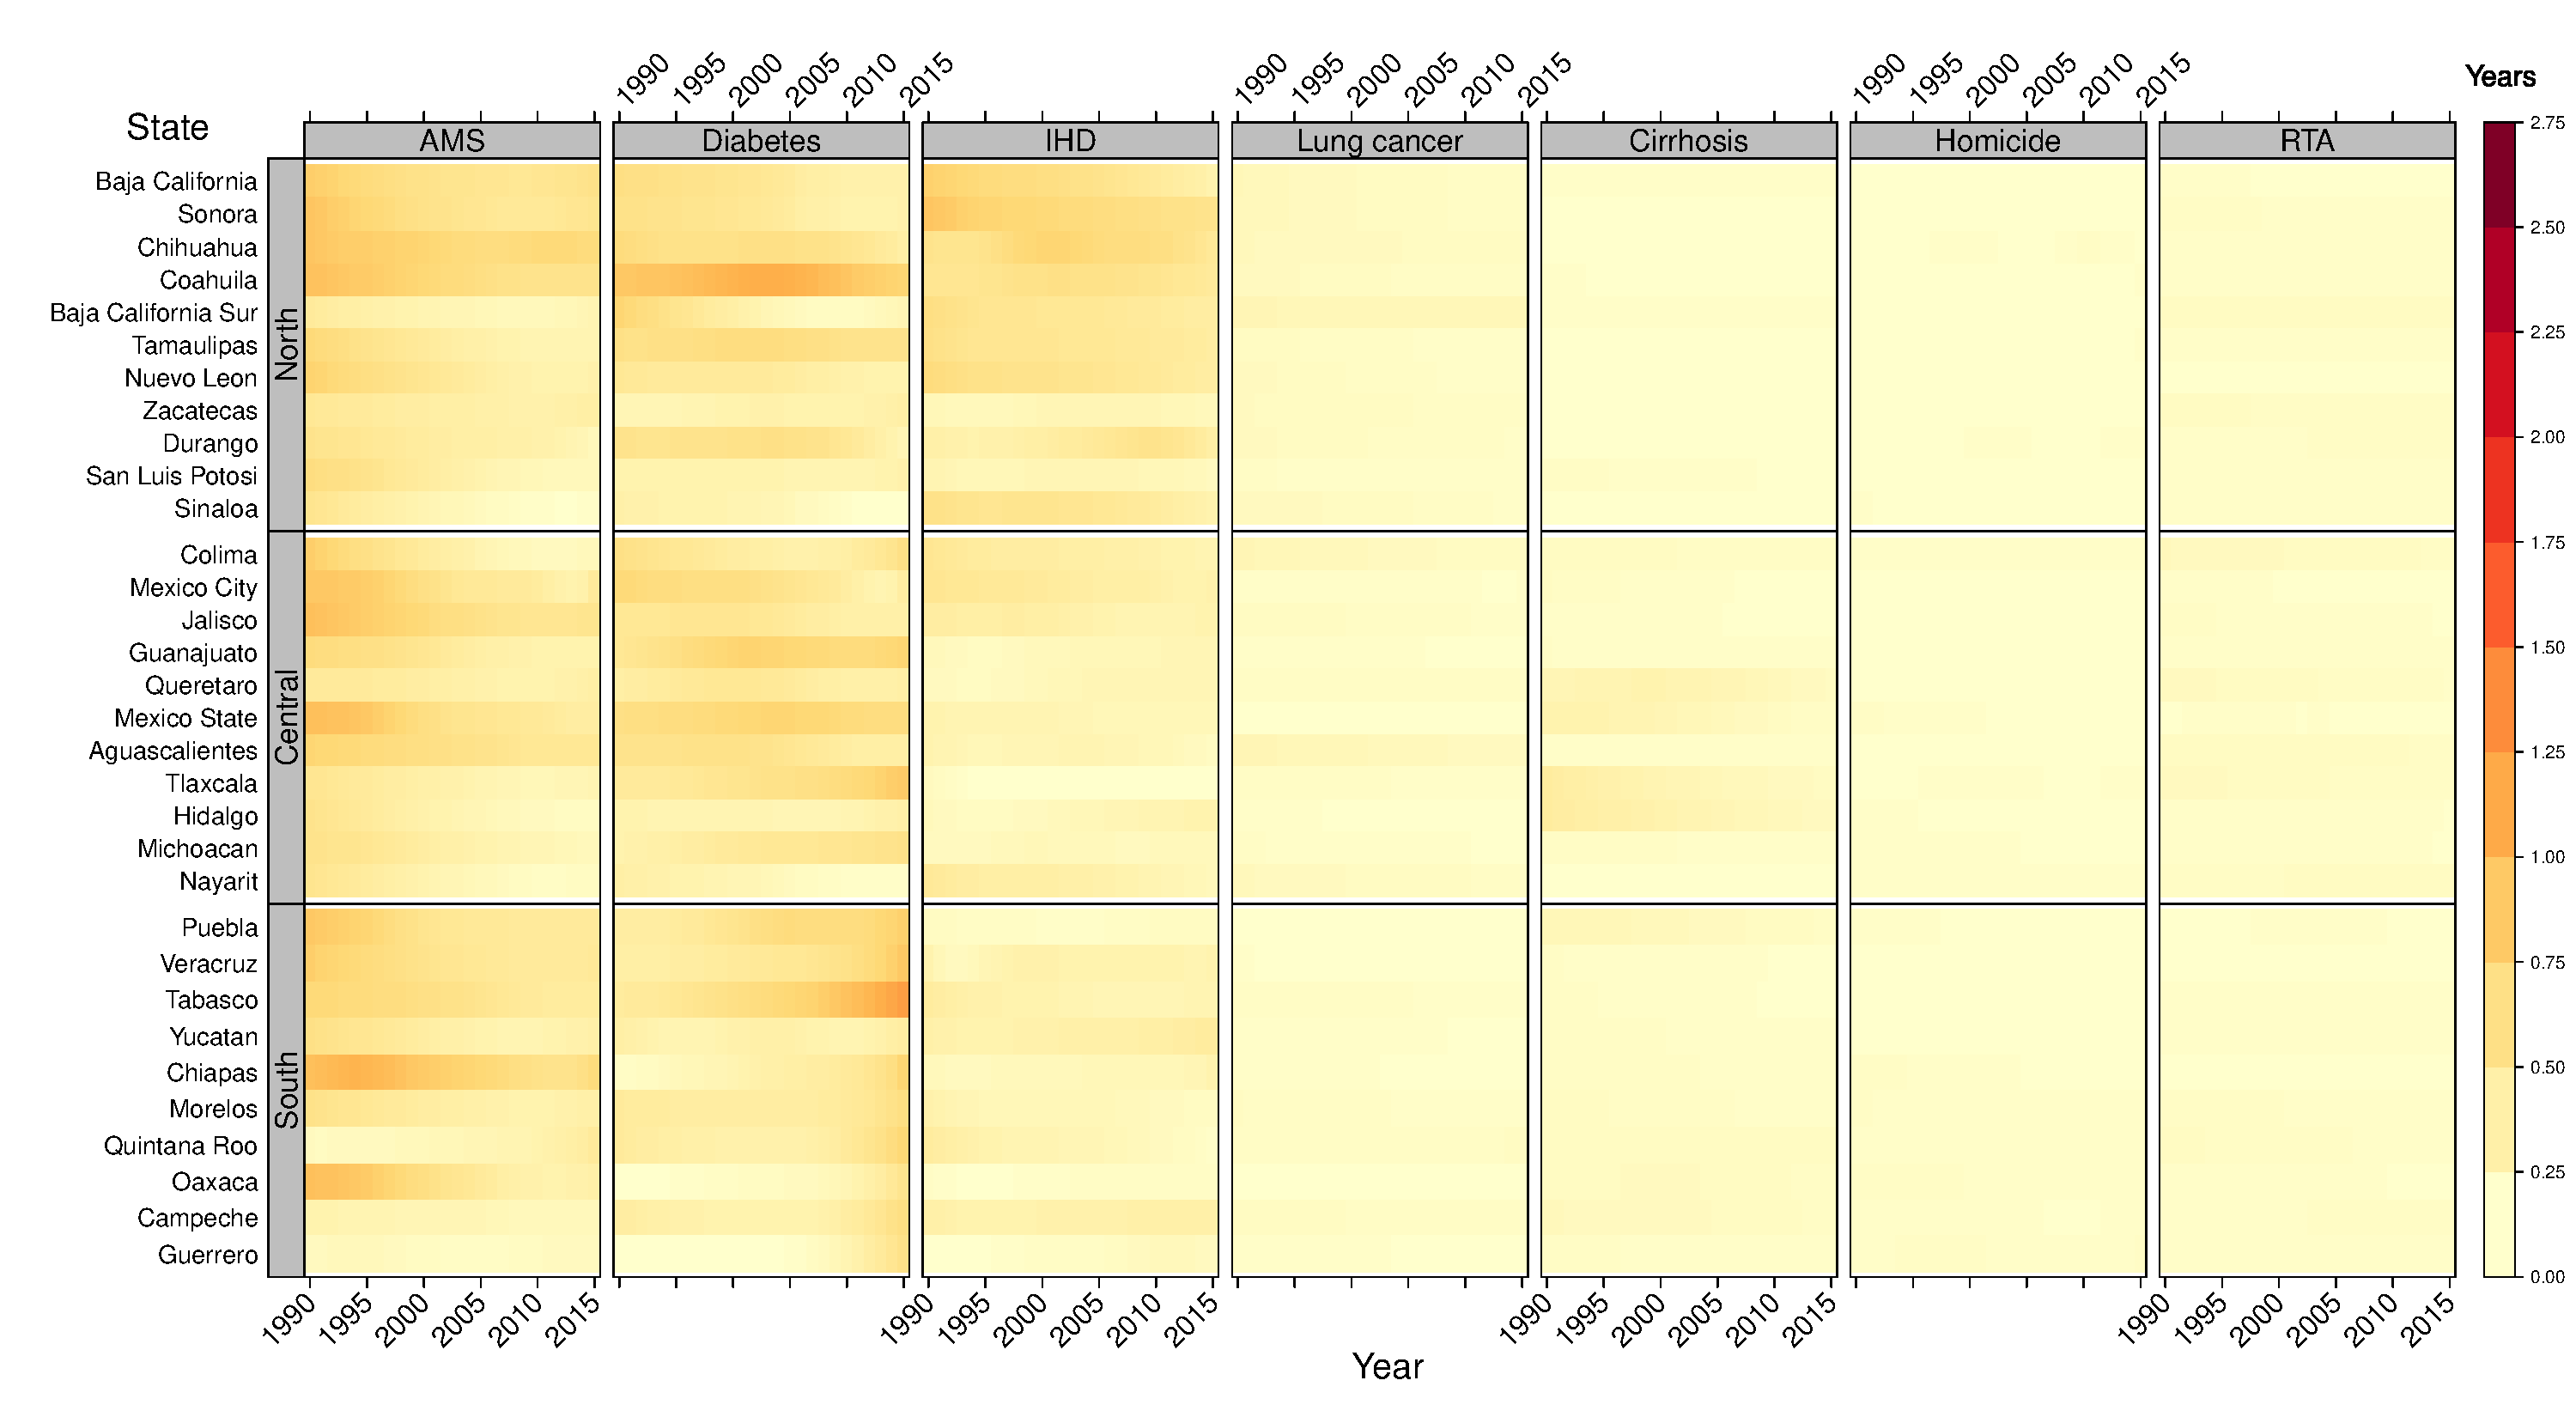
\includegraphics[scale=.30]{Figures/Adult_Female_heatmap.pdf}
Note: AMS is ``amenable to medical service'', IHD is ``isquemic heart diseases'', and RTA is ``road traffic accidents''. Source: own calculations. \end{figure}


\begin{figure}
\centering
\caption{Cause-specific contributions to state differences from low mortality benchmark for male youngest population (ages 0-14), 1990-2015.}
\label{fig:e0_14_males}
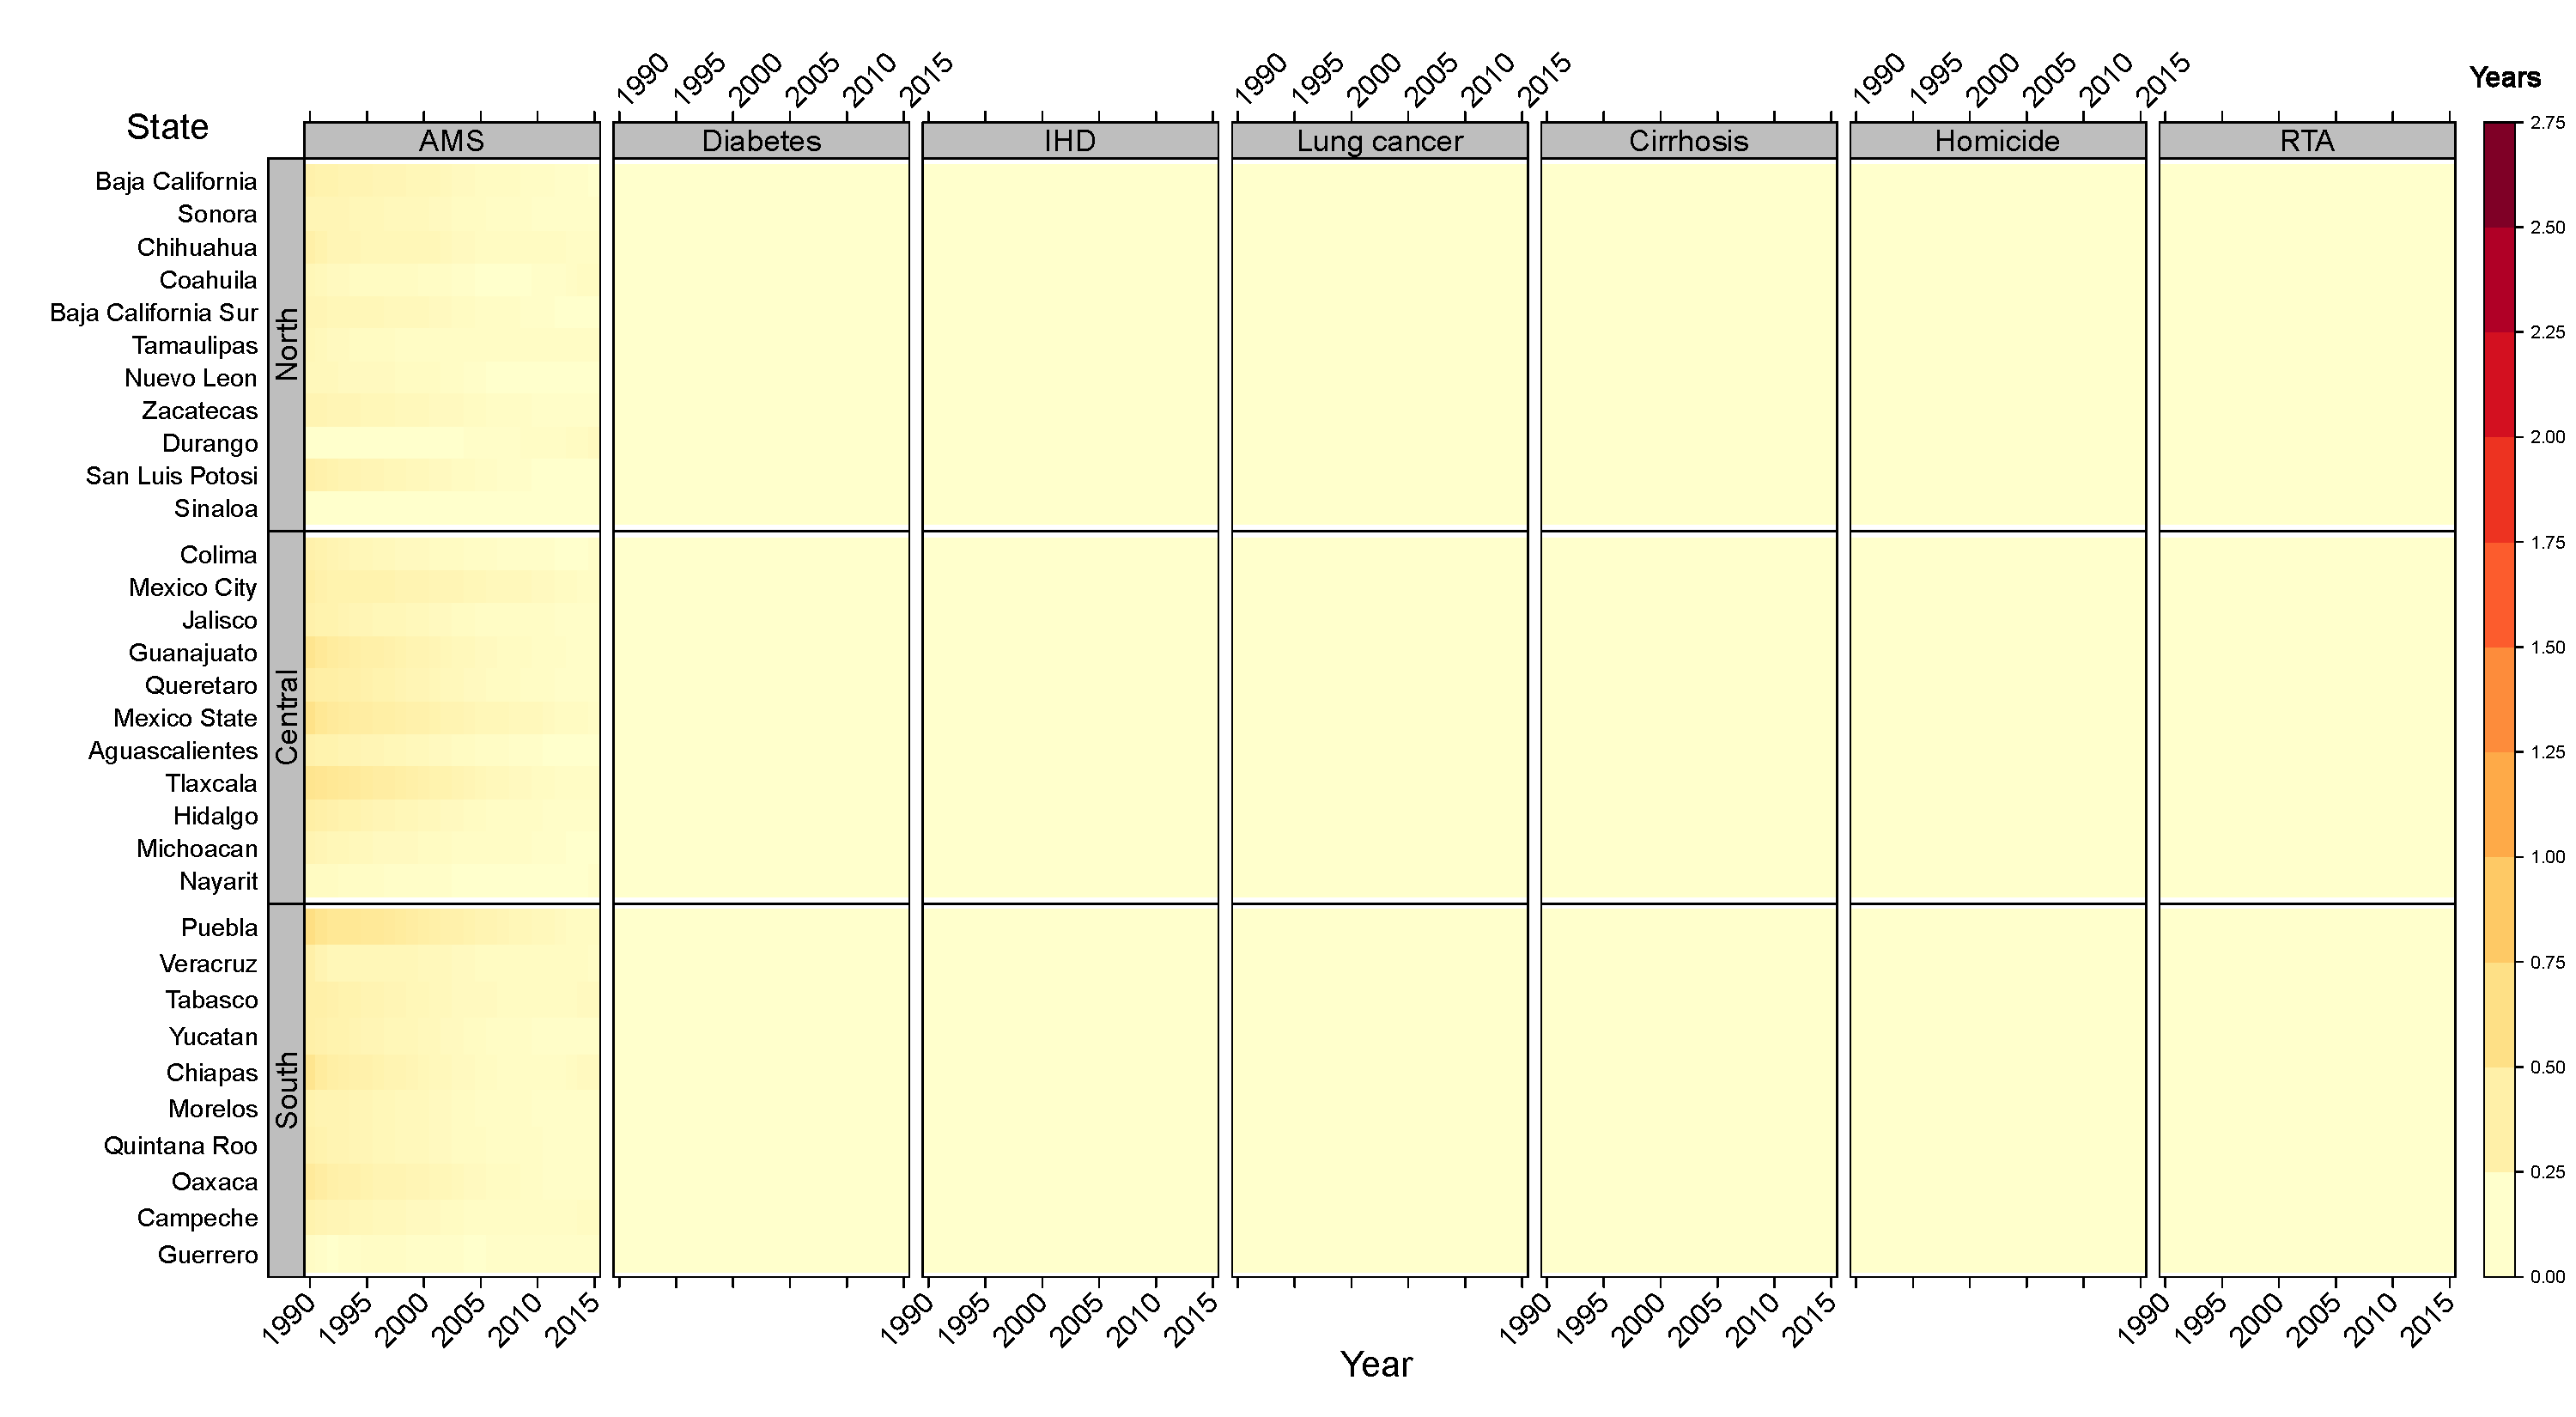
\includegraphics[scale=.3]{Figures/Young_Male_heatmap.pdf}

Note: AMS is ``amenable to medical service'', IHD is ``isquemic heart diseases'', and RTA is ``road traffic accidents''. Source: own calculations.\end{figure}

\begin{figure}
\centering
\caption{Cause-specific contributions to state differences from low mortality benchmark for female youngest population (ages 0-14), 1990-2015.} 
\label{fig:e0_14_females}
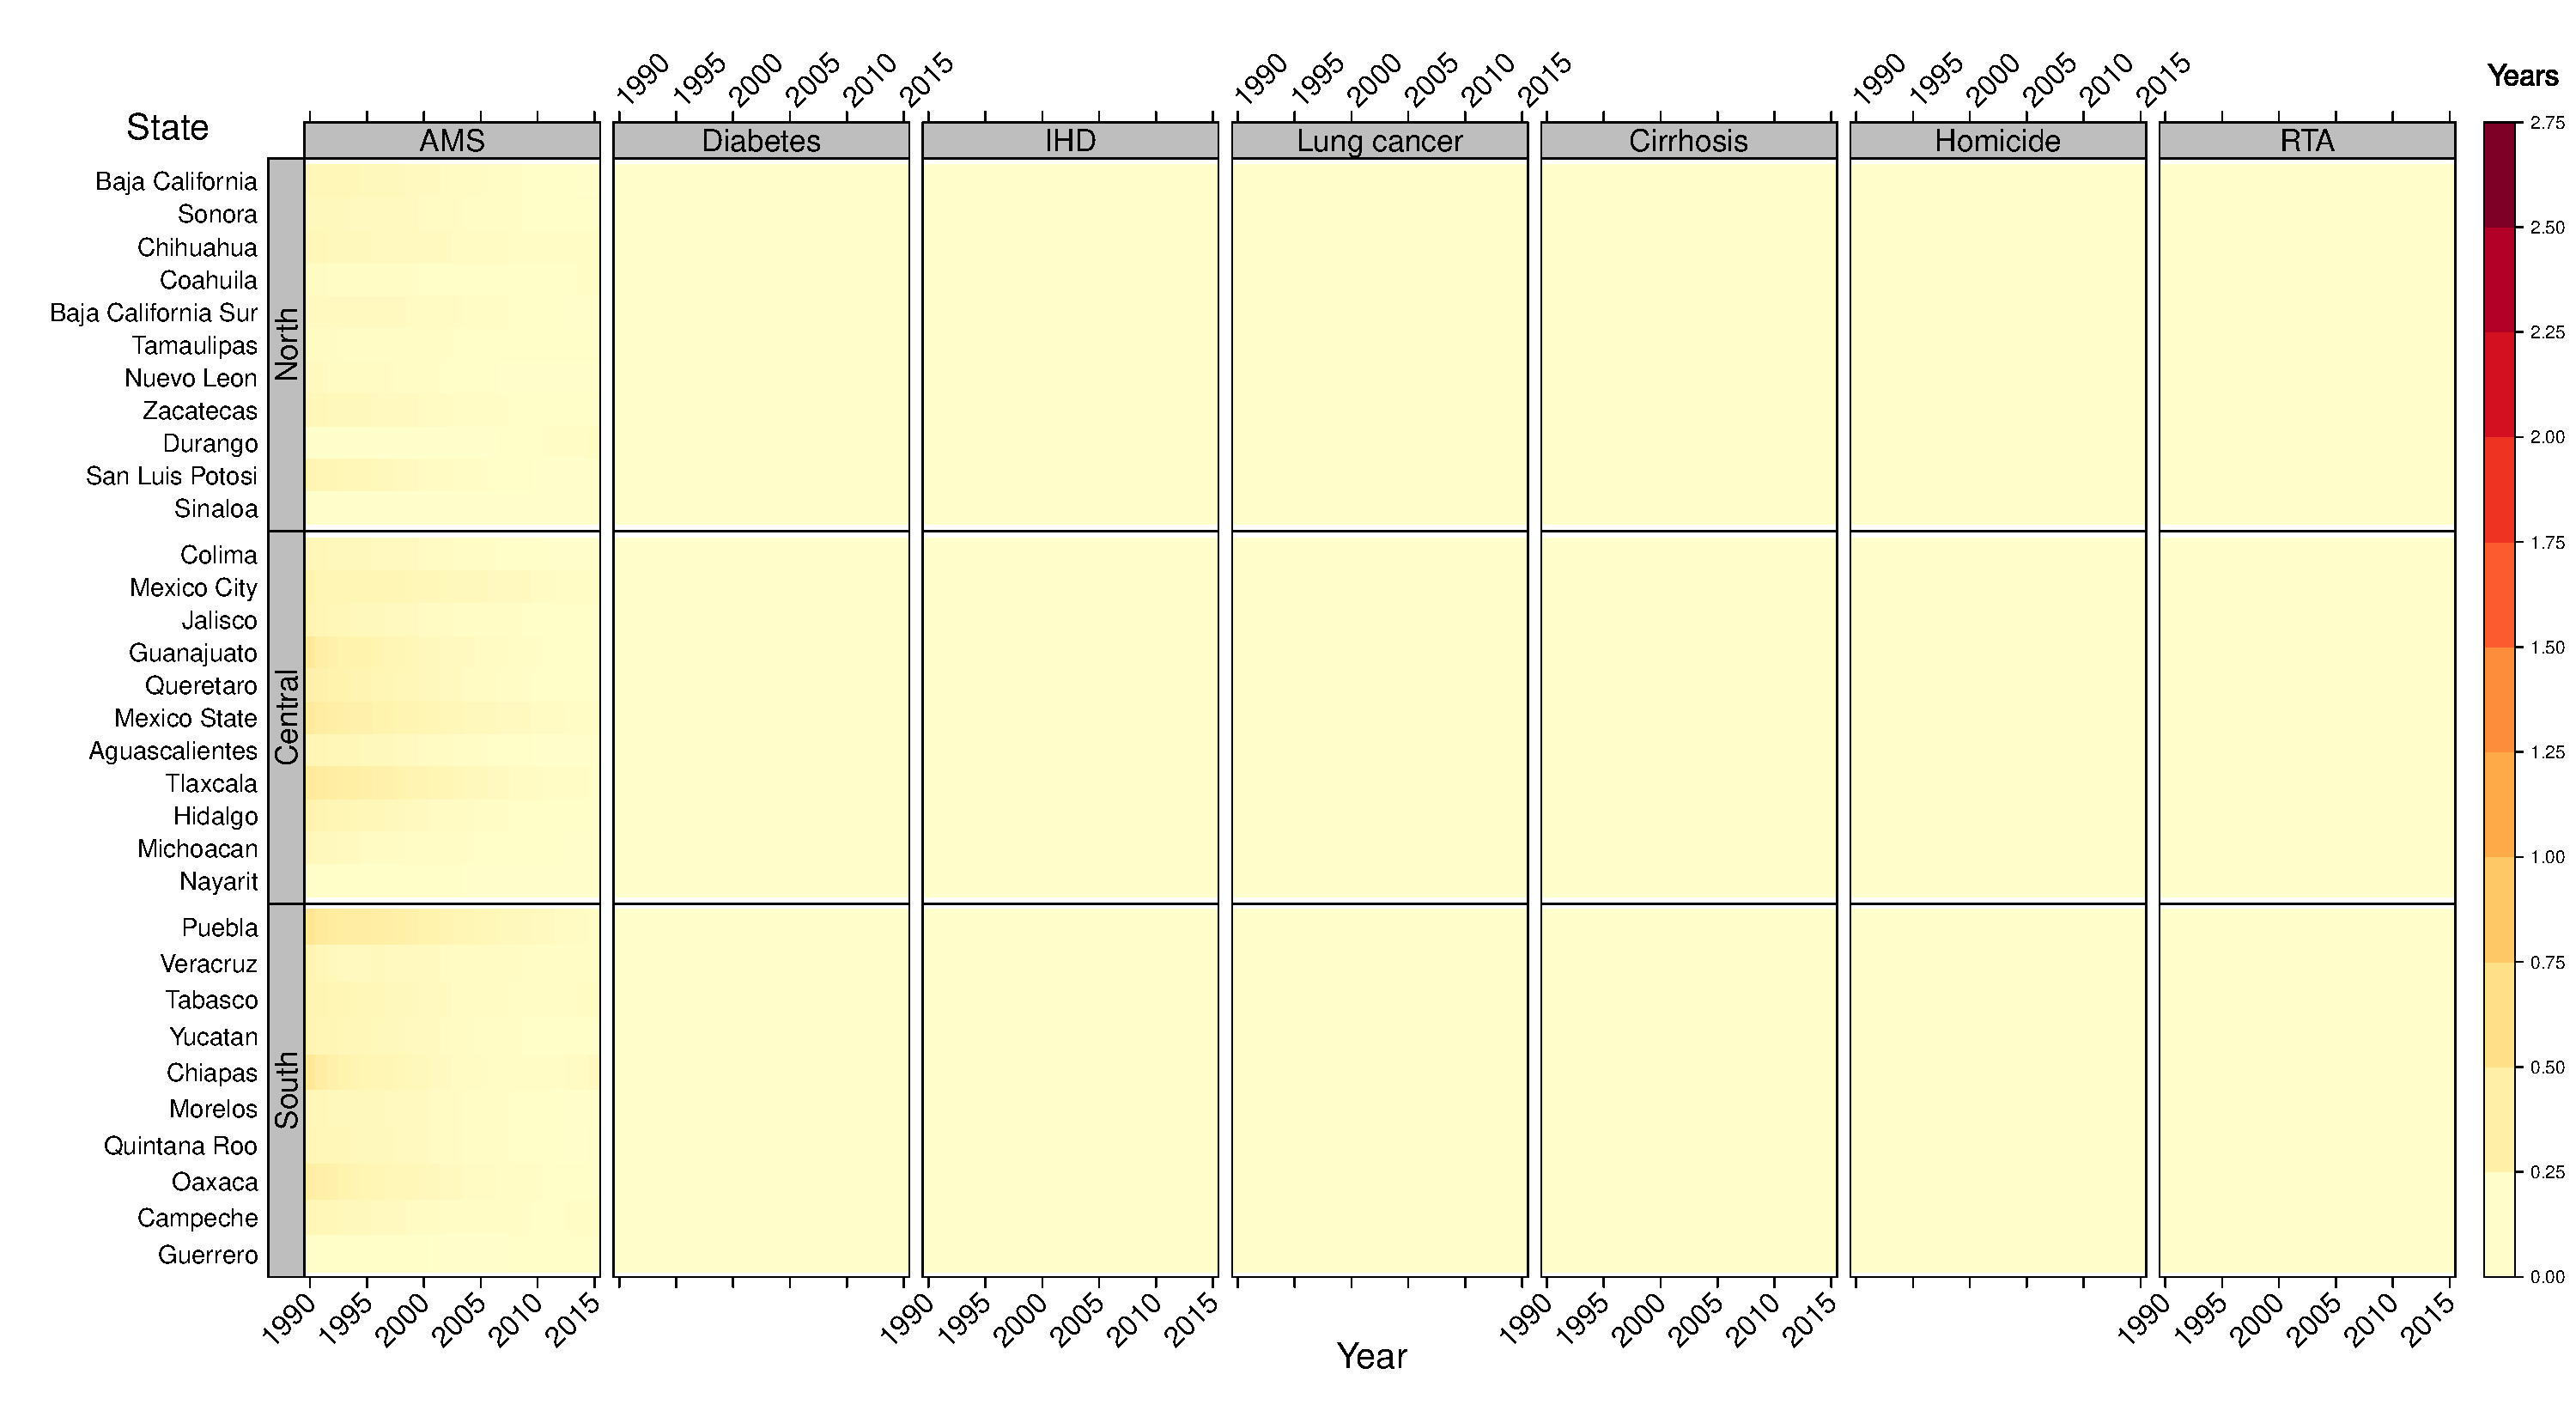
\includegraphics[scale=.3]{Figures/Young_Female_heatmap.pdf}

Note: AMS is ``amenable to medical service'', IHD is ``isquemic heart diseases'', and RTA is ``road traffic accidents''. Source: own calculations.
\end{figure}


\begin{figure}
\centering
\caption{Cause-specific contributions to state differences from low mortality benchmark for male young adults (ages 15-49), 1990-2015.}
\label{fig:e15_39_males}
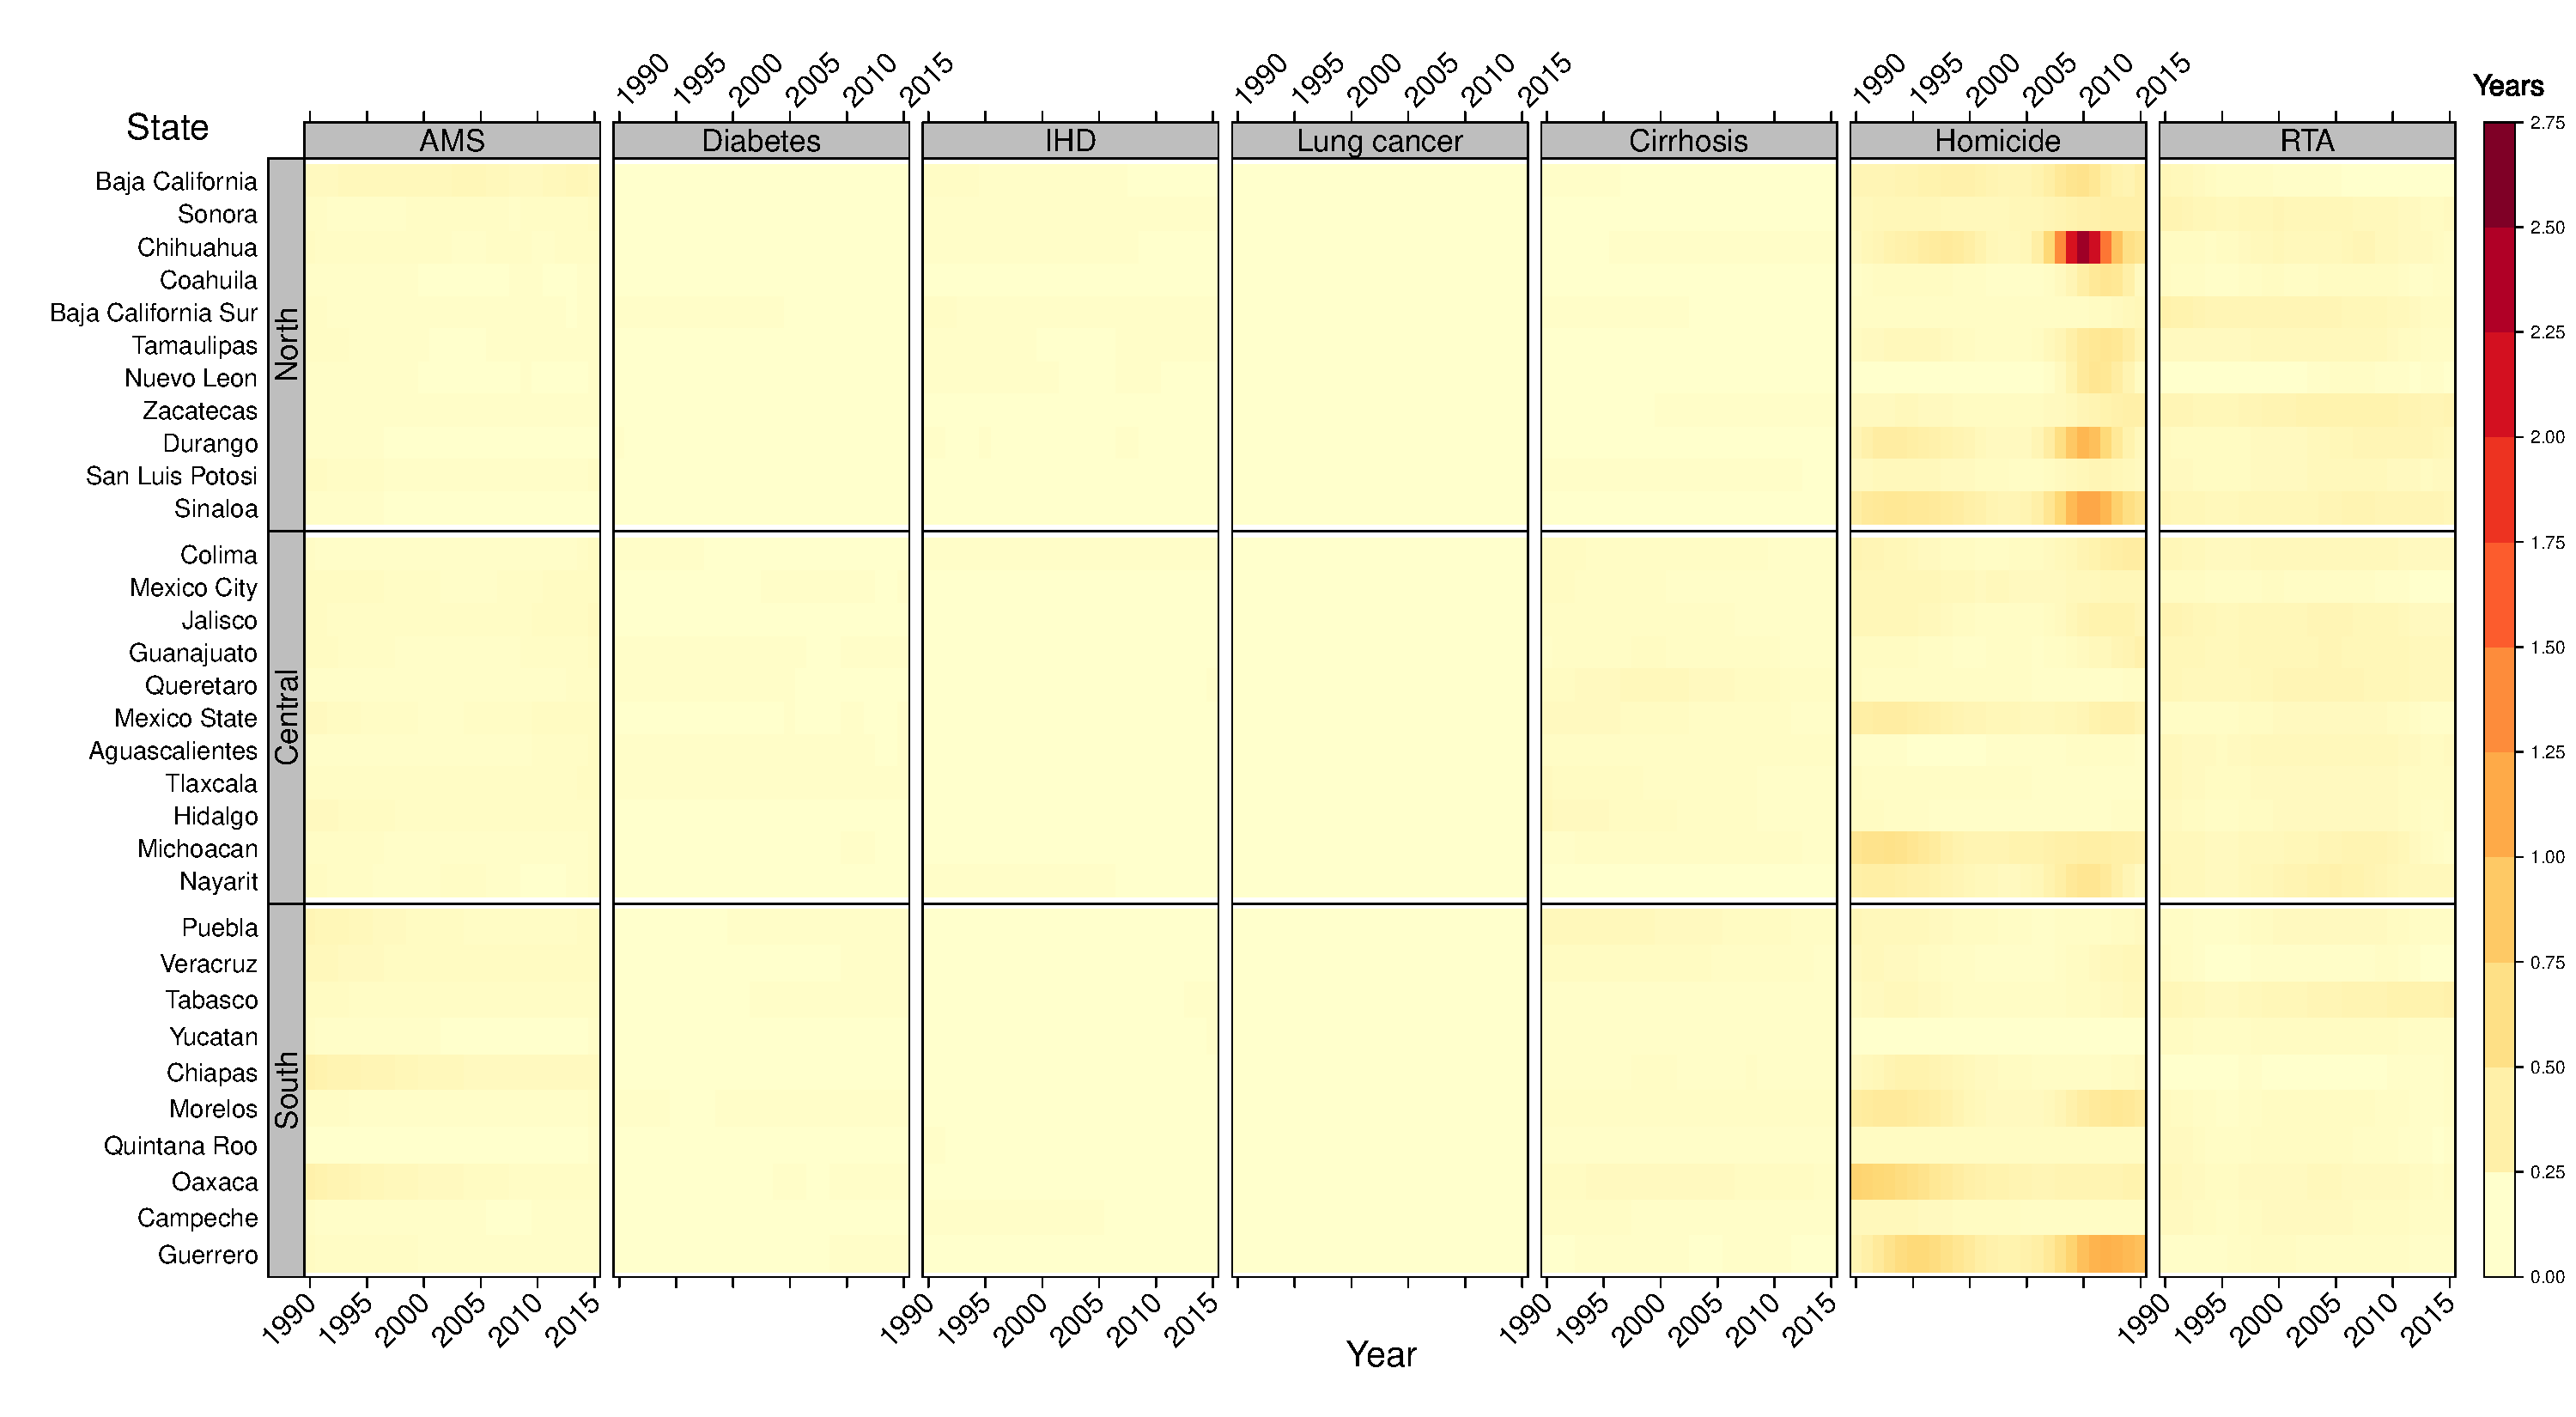
\includegraphics[scale=.3]{Figures/YoungAdult_Male_heatmap.pdf}
Note: AMS is ``amenable to medical service'', IHD is ``isquemic heart diseases'', and RTA is ``road traffic accidents''. Source: own calculations.
\end{figure}

\begin{figure}
\centering
\caption{Cause-specific contributions to state differences from low mortality benchmark for female young adults (ages 15-49), 1990-2015.}
\label{fig:e15_39_females}
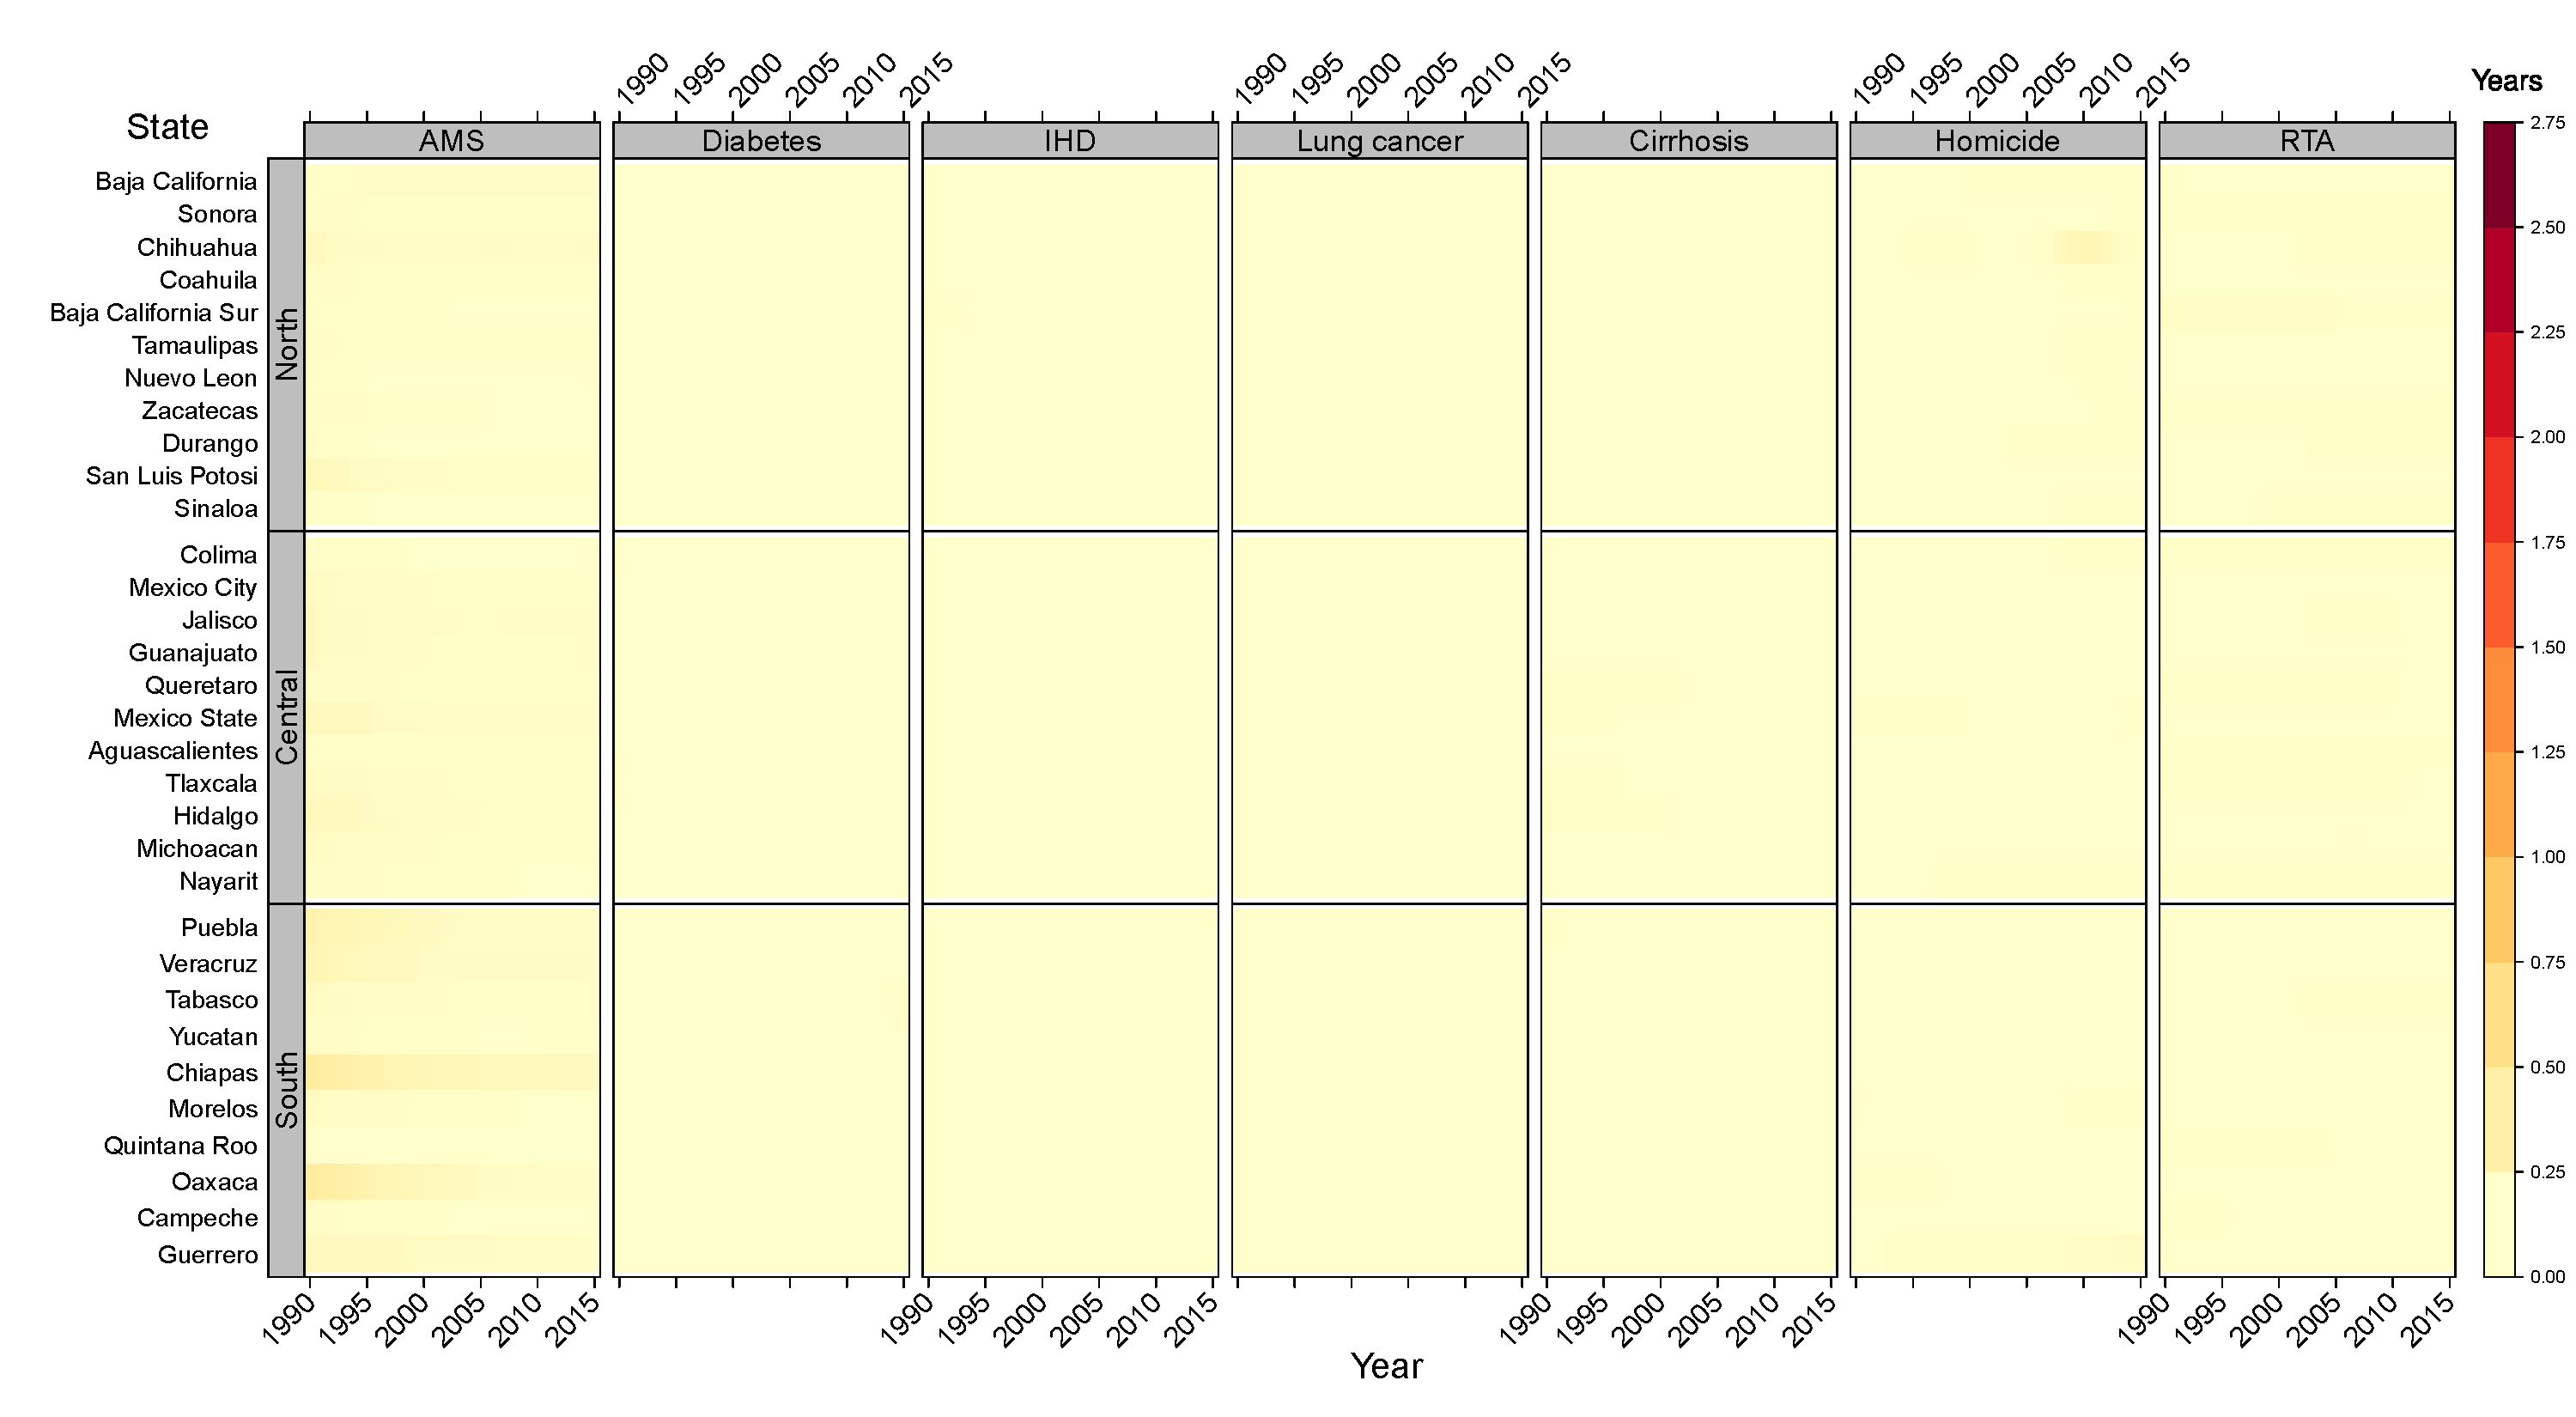
\includegraphics[scale=.3]{Figures/YoungAdult_Female_heatmap.pdf}
Note: AMS is ``amenable to medical service'', IHD is ``isquemic heart diseases'', and RTA is ``road traffic accidents''. Source: own calculations.
\end{figure}



\begin{figure}
\centering
\caption{State specific gap with low mortality benchmark for selected years between ages 0-14. Source: own calculations.}
\begin{center}
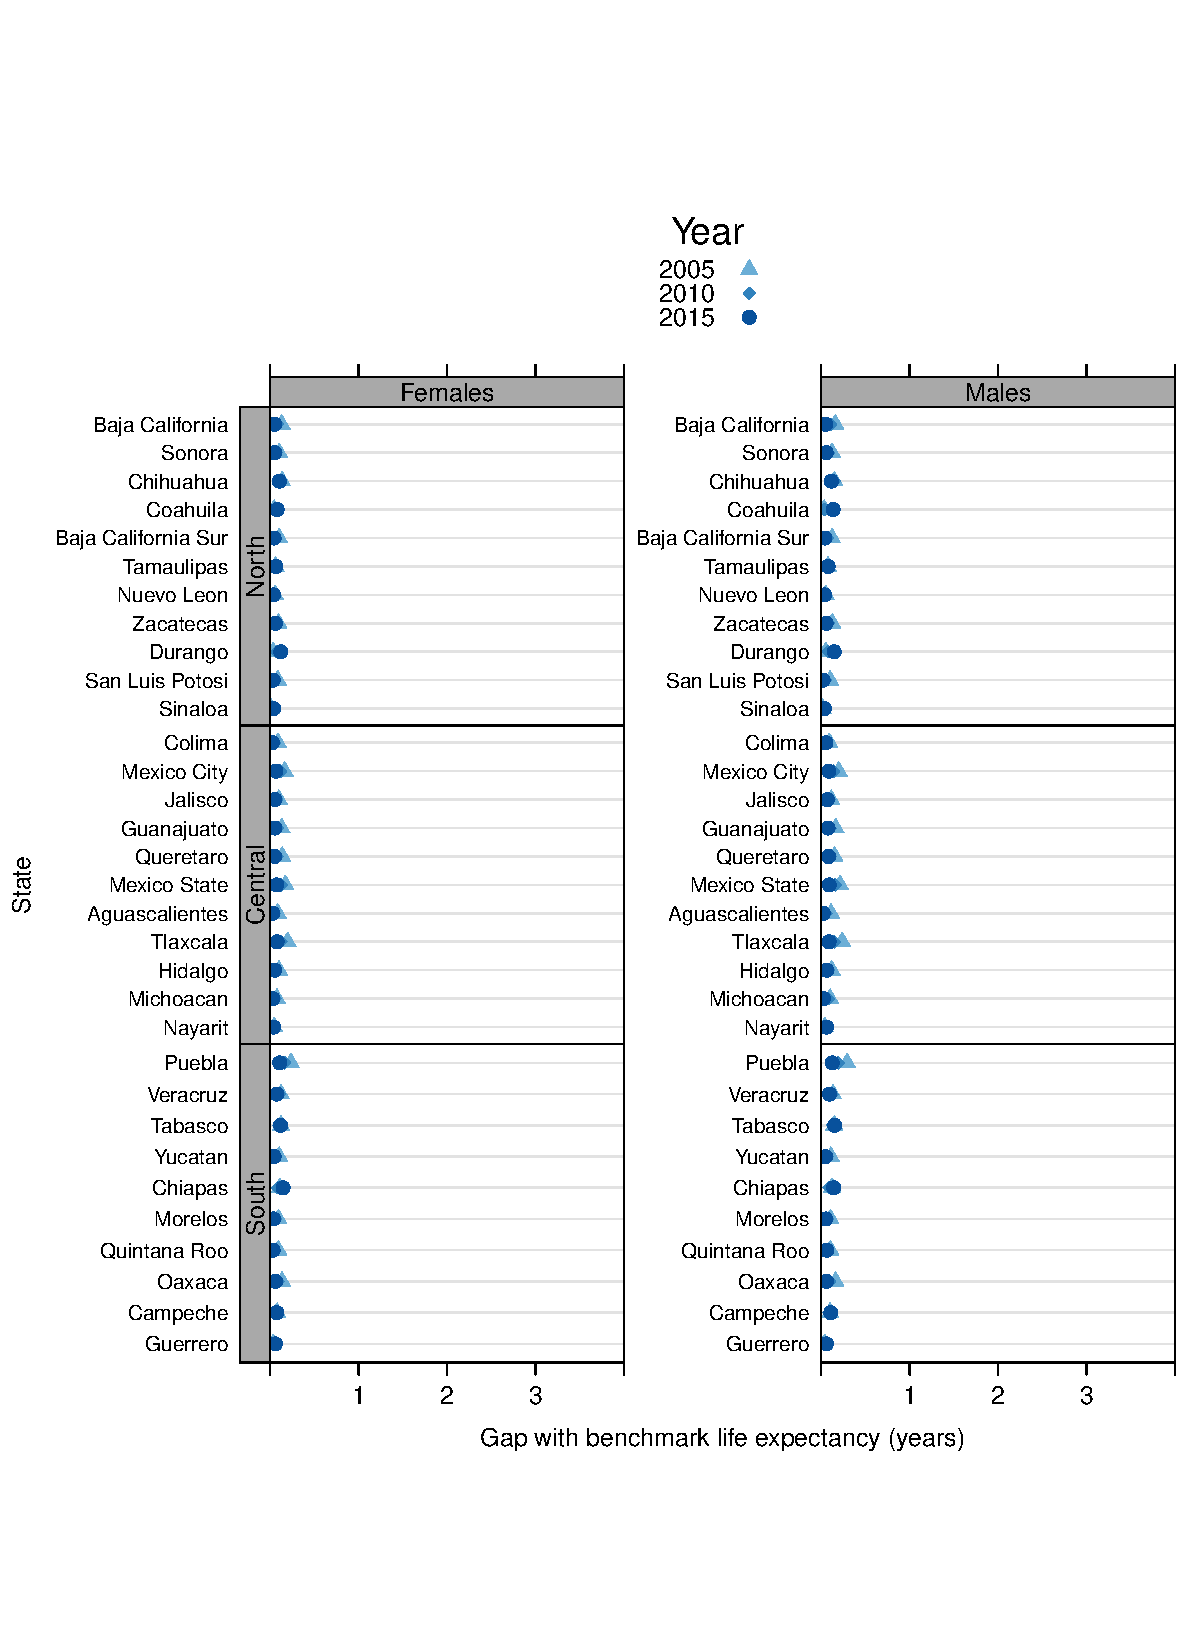
\includegraphics[scale=.8]{Figures/Distance_y.pdf}
\end{center}
\end{figure}

\begin{figure}
\centering
\caption{State specific gap with low mortality benchmark for selected years between ages 15-49. Source: own calculations.}
\begin{center}
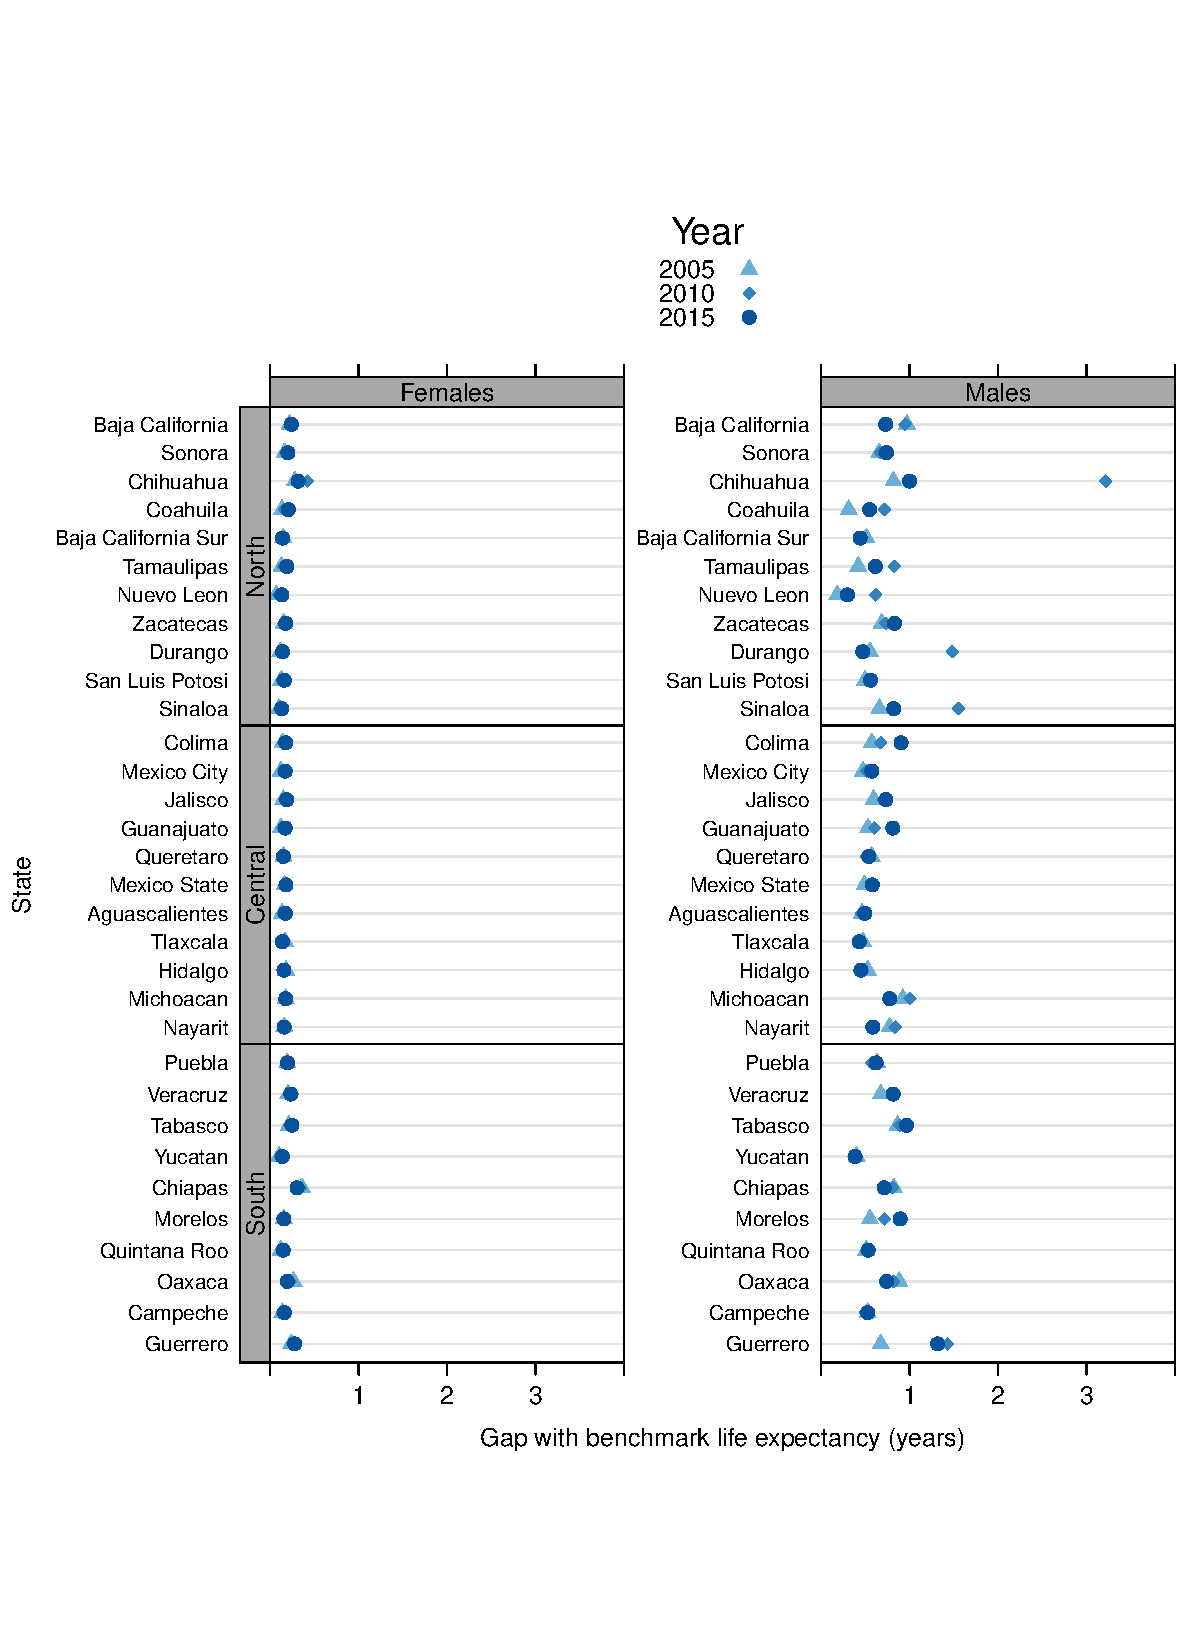
\includegraphics[scale=.8]{Figures/Distance_ya.pdf}
\end{center}
\end{figure}

\begin{figure}
\centering
\caption{State specific gap with low mortality benchmark for selected years between ages 50-84. Source: own calculations.}
\begin{center}
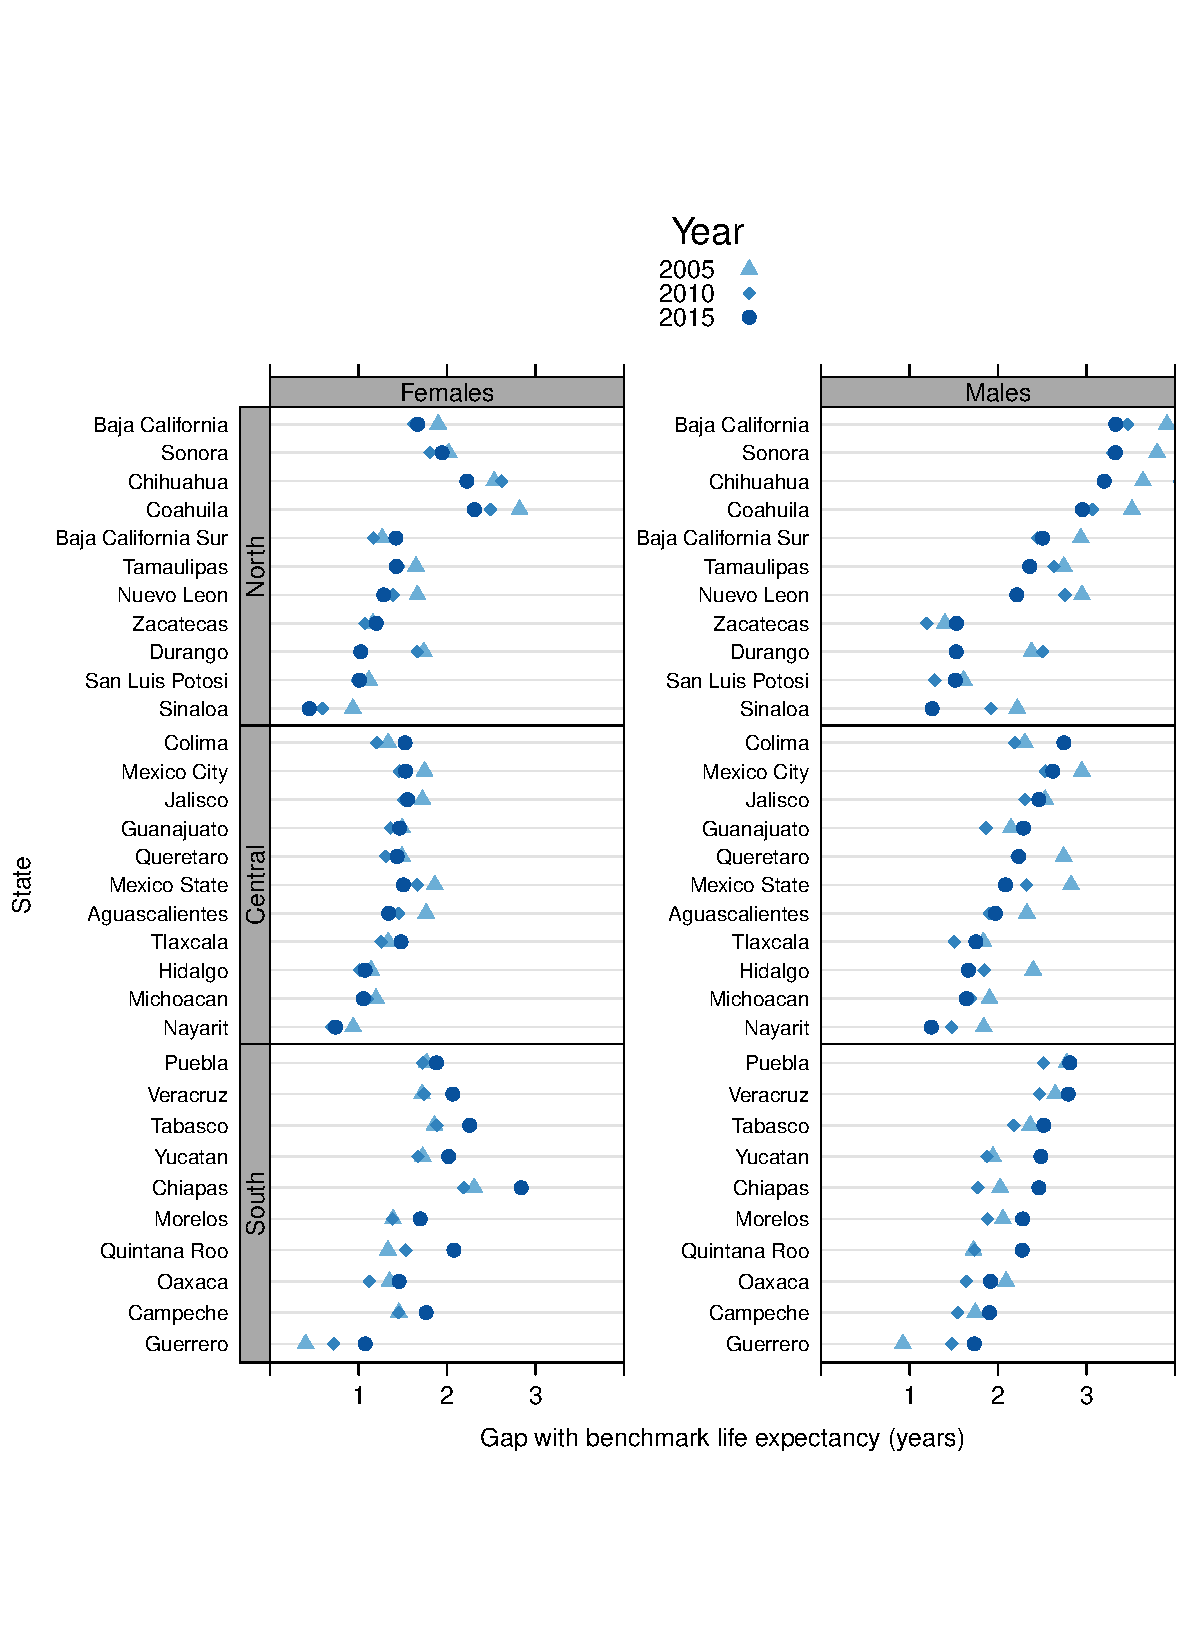
\includegraphics[scale=.8]{Figures/Distance_oa.pdf}
\end{center}
\end{figure}






\begin{figure}
\centering
\caption{Proportion by cause of death from benchmark mortality for youngest females (ages 0-14). Source: own calculations.}
\begin{center}
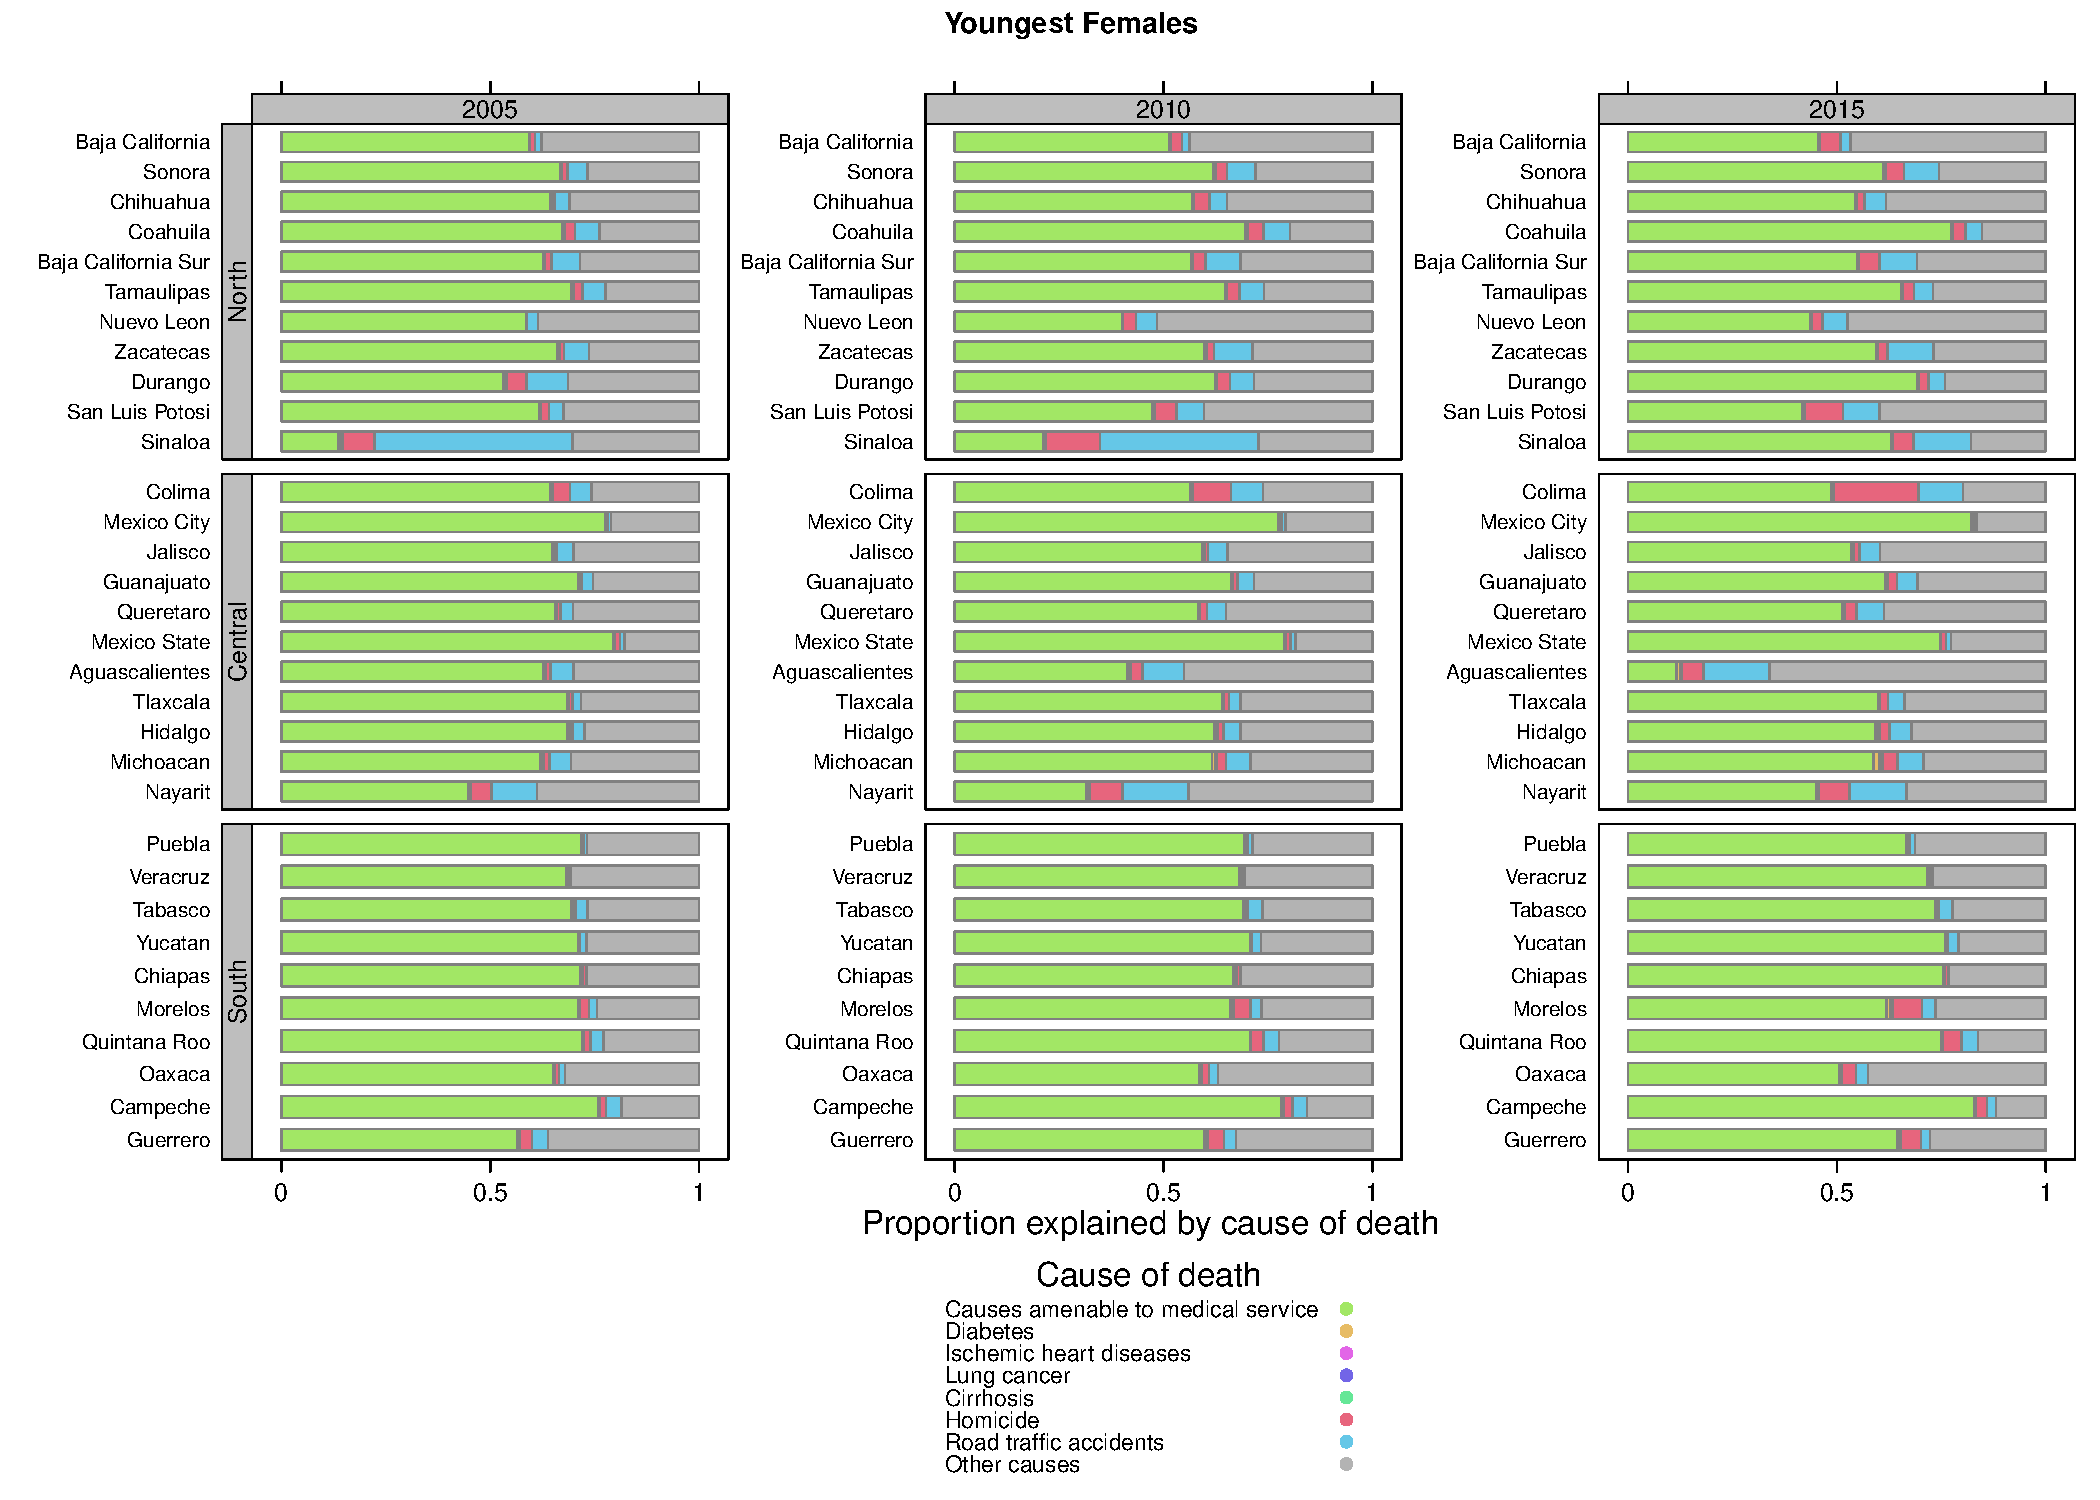
\includegraphics[scale=.5]{Figures/Figure_prop_yf.pdf}
\end{center}
\end{figure}

\begin{figure}
\centering
\caption{Proportion by cause of death from benchmark mortality for youngest males (ages 0-14). Source: own calculations.}
\begin{center}
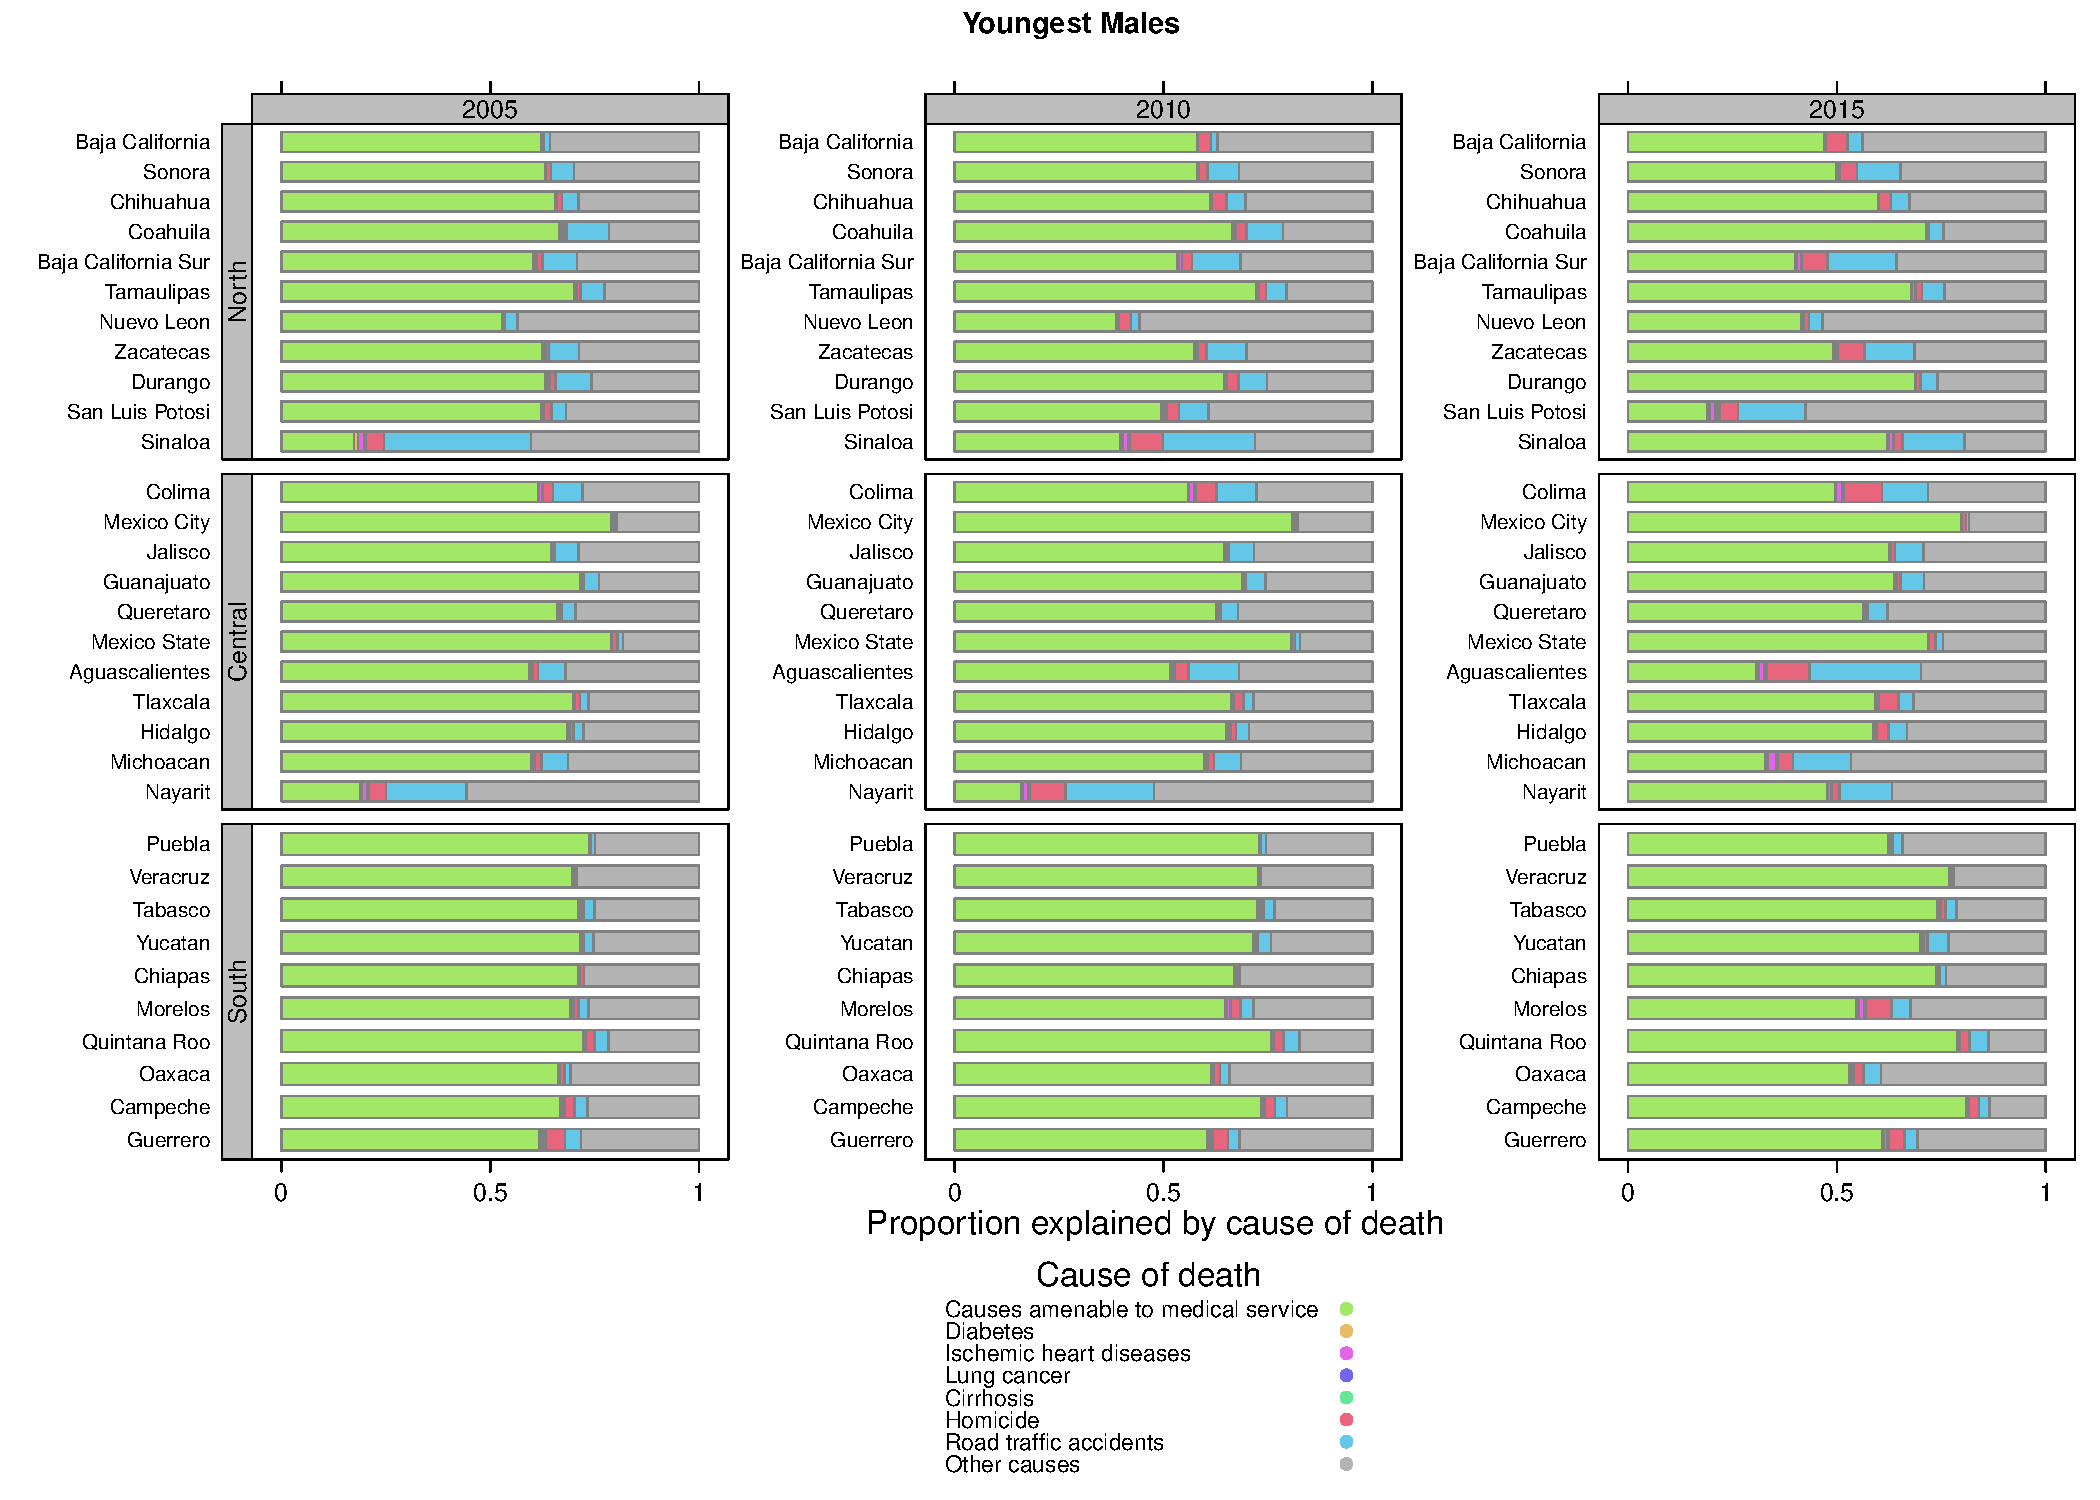
\includegraphics[scale=.5]{Figures/Figure_prop_ym.pdf}
\end{center}
\end{figure}



\begin{figure}
\centering
\caption{Proportion by cause of death from benchmark mortality for young adult females (ages 15-49). Source: own calculations.}
\begin{center}
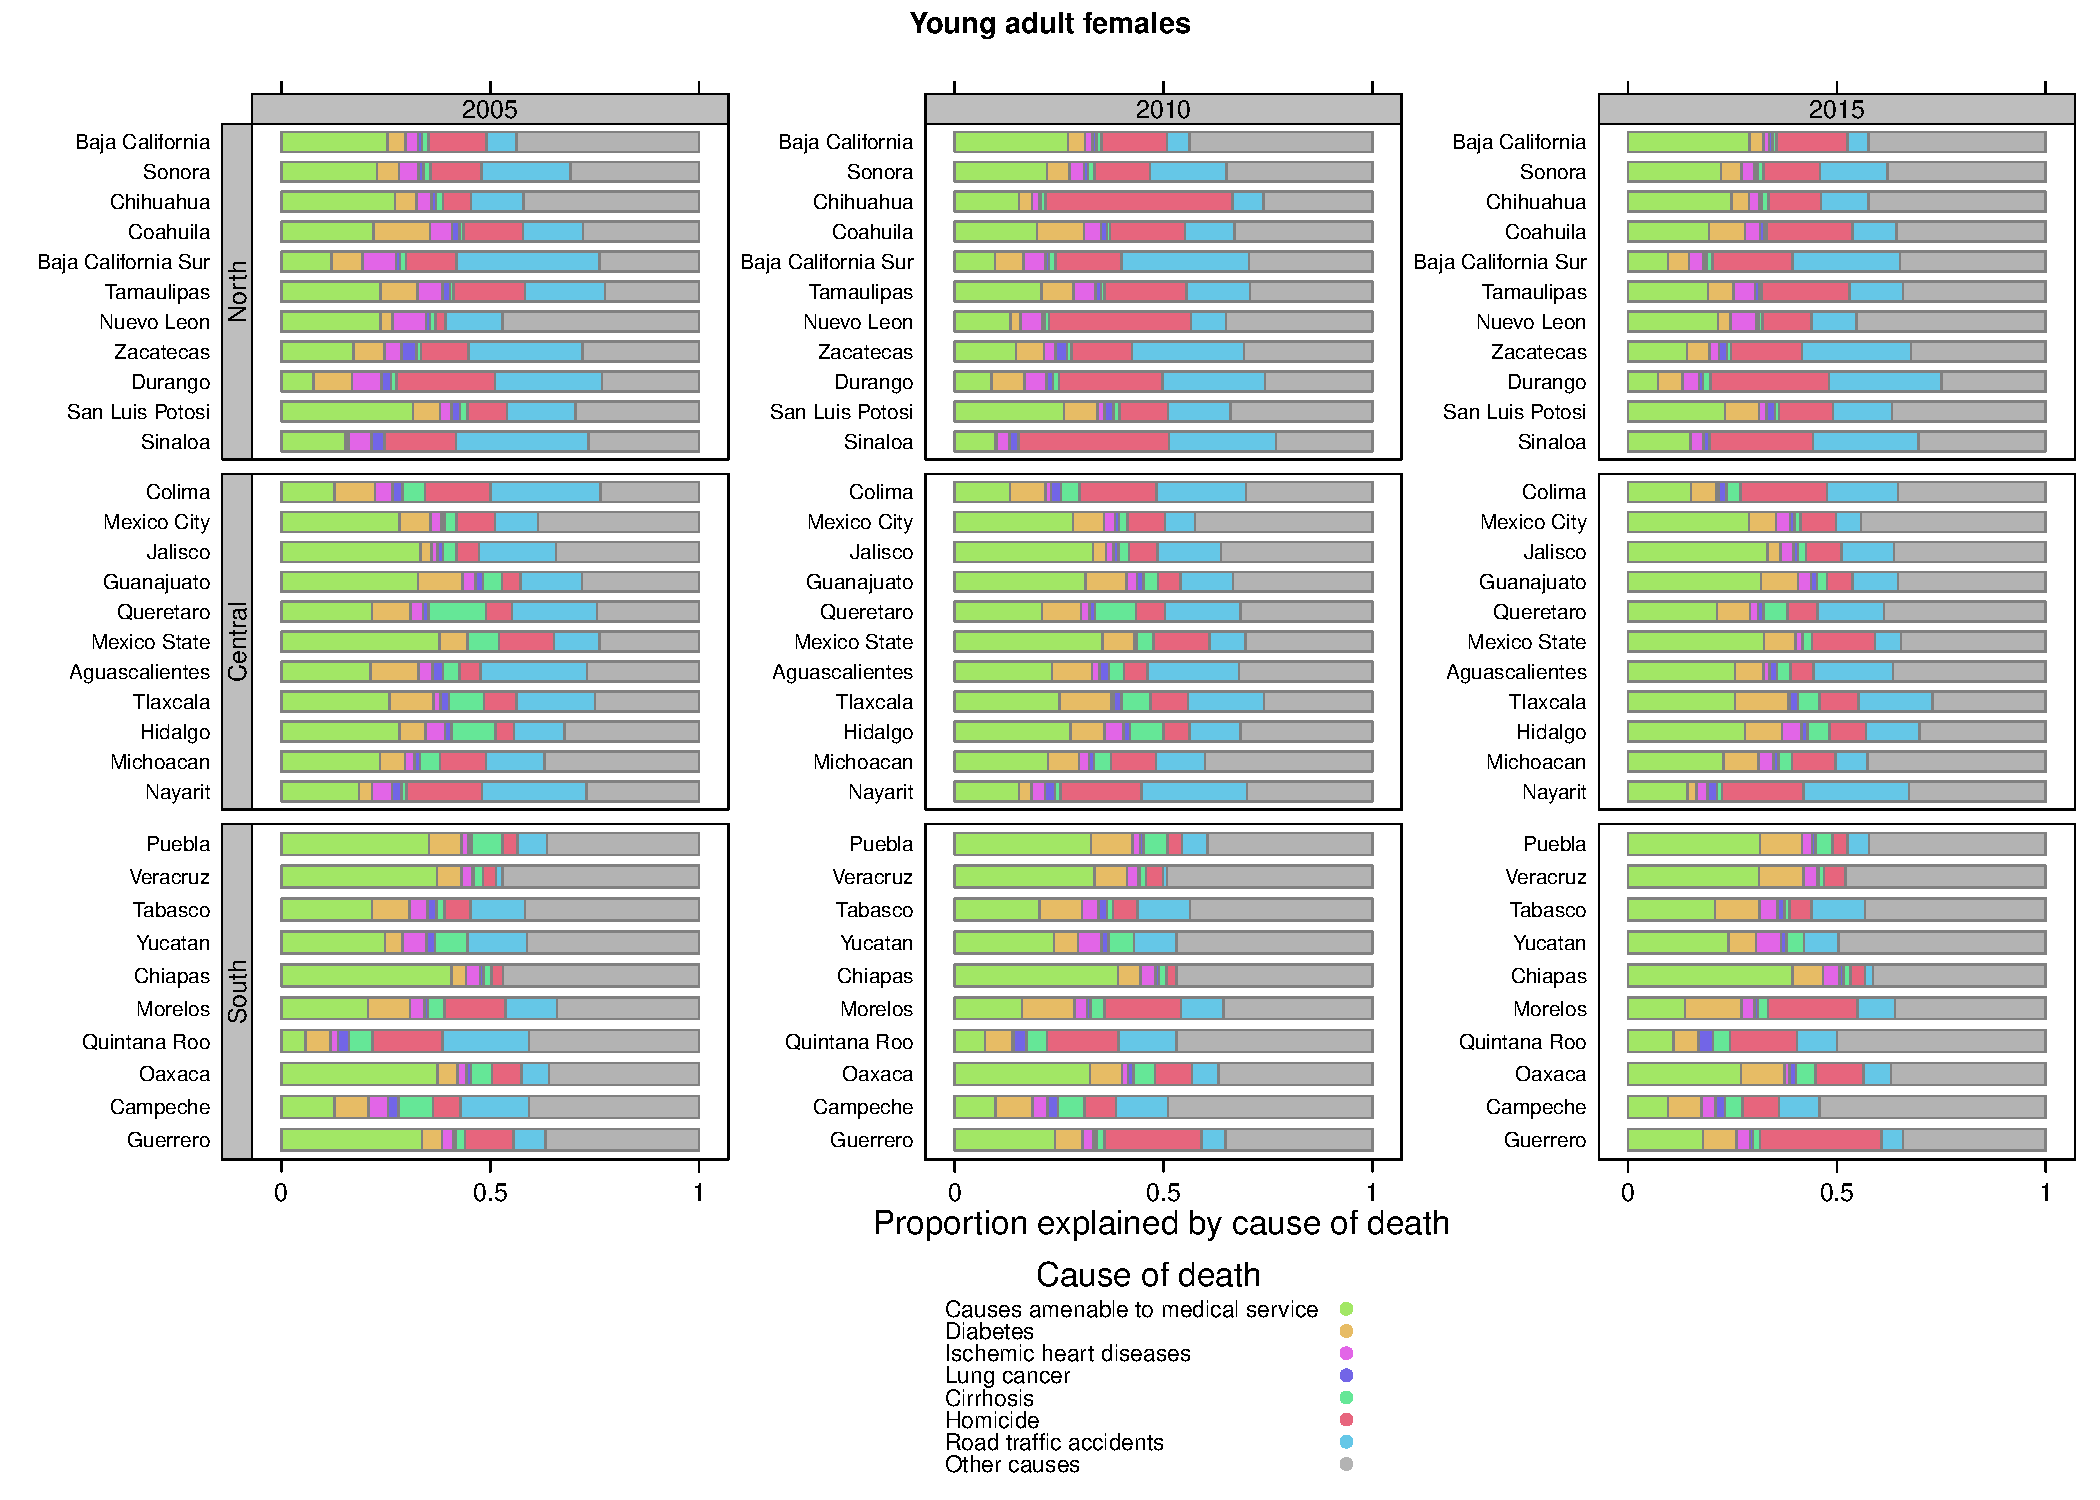
\includegraphics[scale=.5]{Figures/Figure_prop_yaf.pdf}
\end{center}
\end{figure}


\begin{figure}
\centering
\caption{Proportion by cause of death from benchmark mortality for young adult males (ages 15-49). Source: own calculations.}
\begin{center}
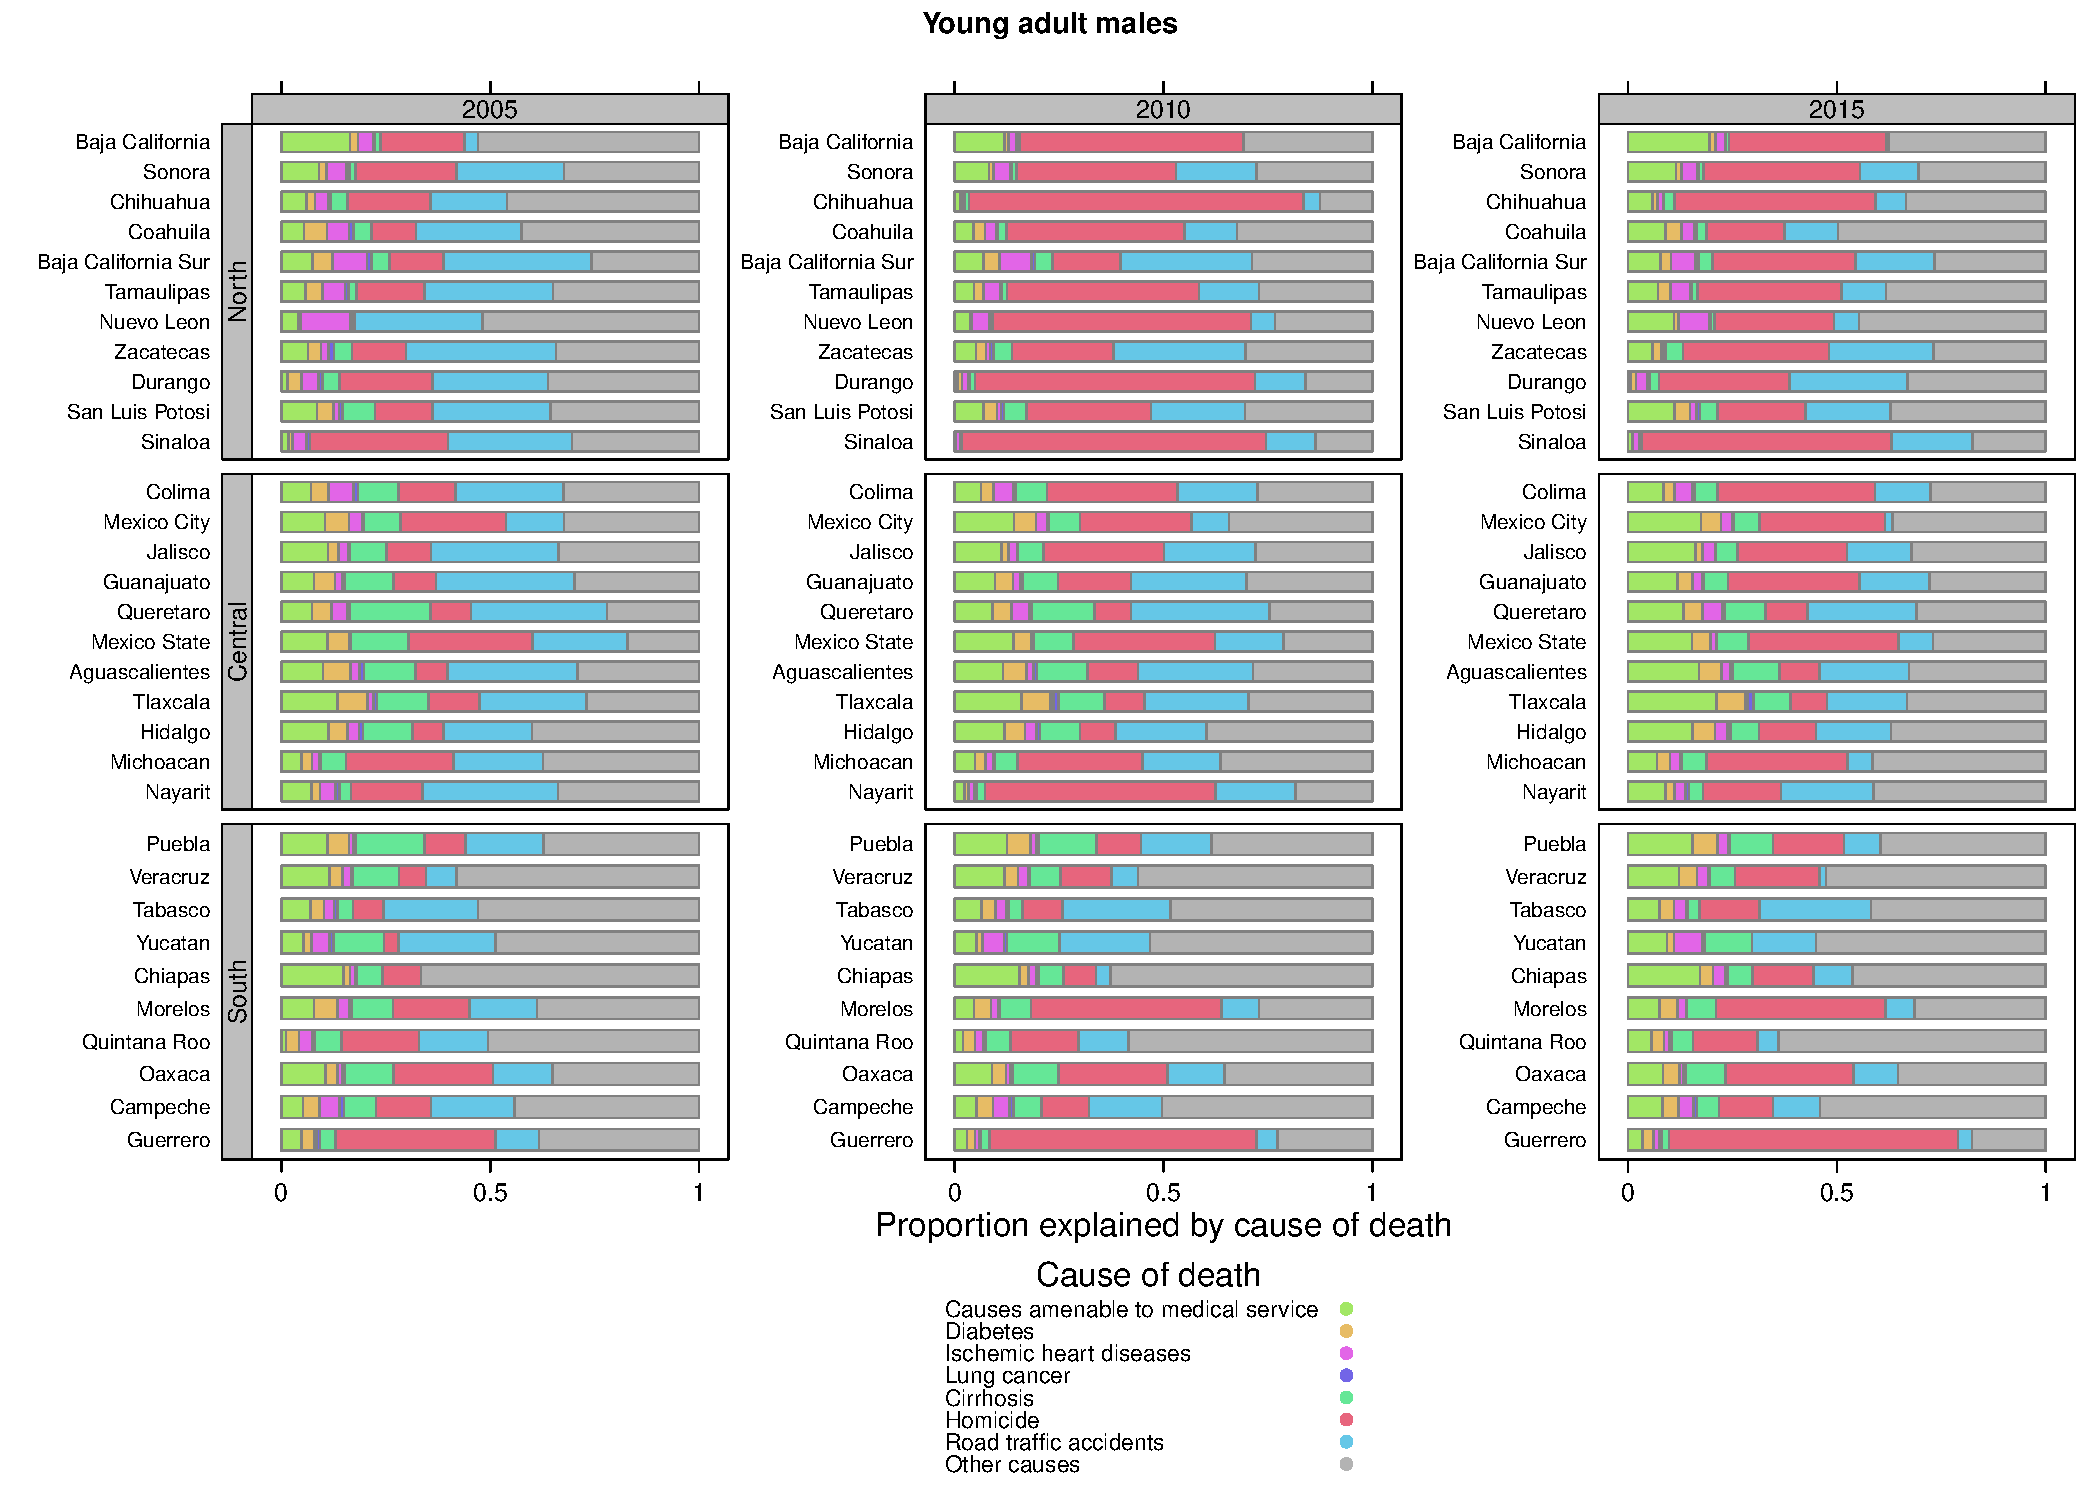
\includegraphics[scale=.5]{Figures/Figure_prop_yam.pdf}
\end{center}
\end{figure}


\begin{figure}
\centering
\caption{Proportion by cause of death from benchmark mortality for older male adults (ages 50-84). Source: own calculations.}
\begin{center}
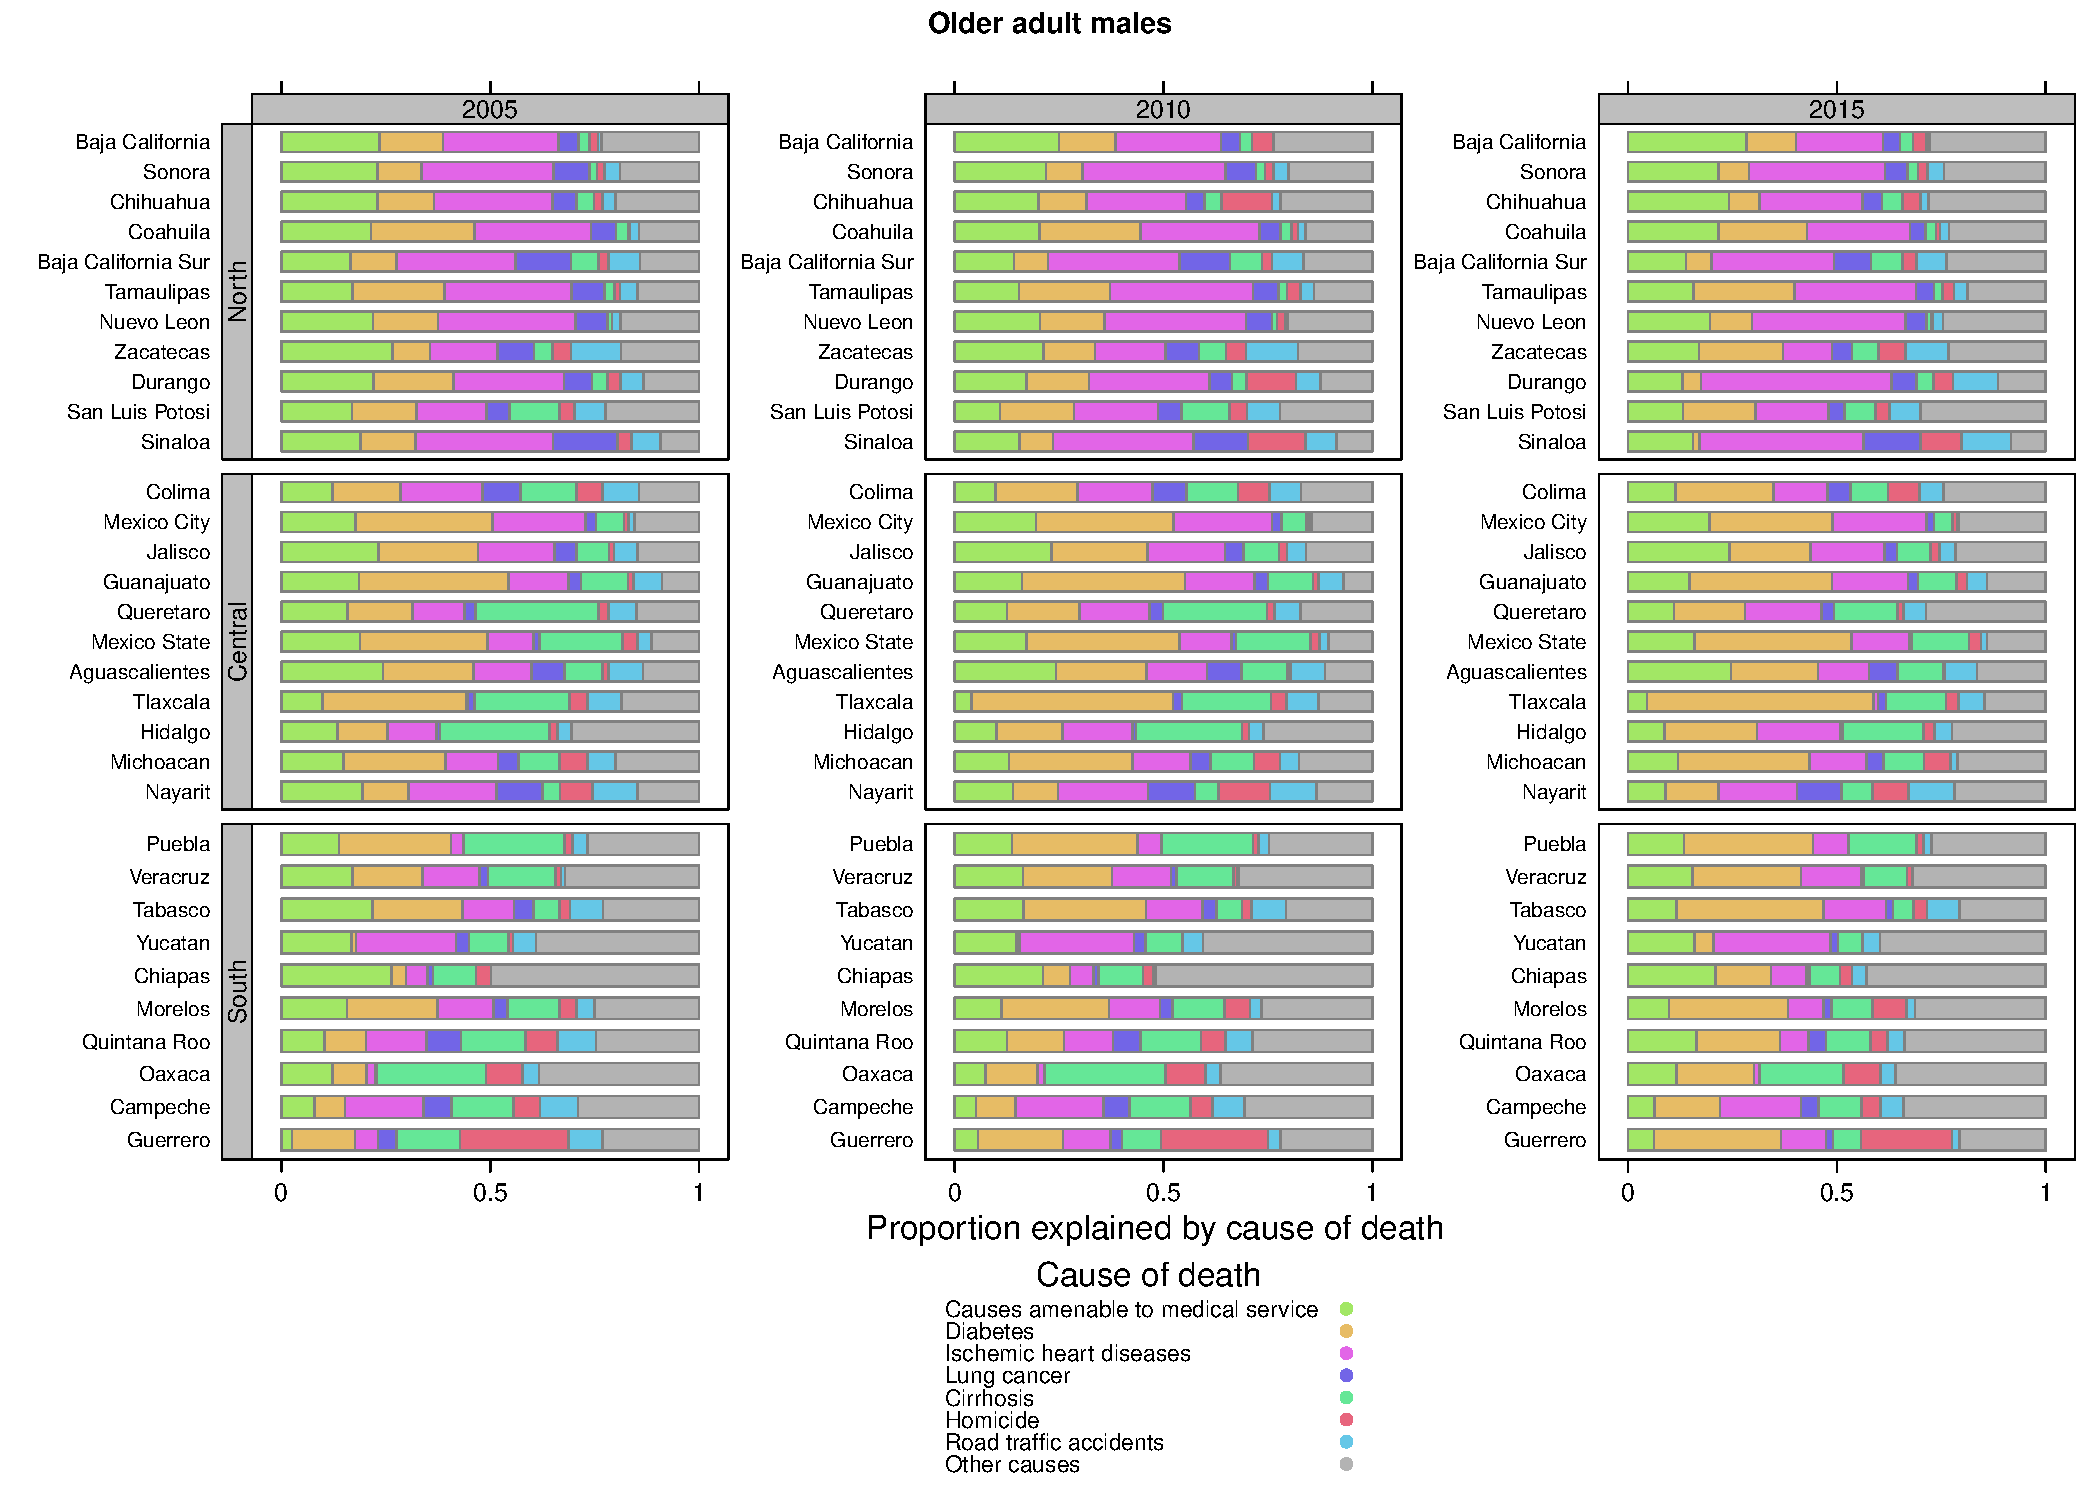
\includegraphics[scale=.5]{Figures/Figure_prop_oam.pdf}
\end{center}
\end{figure}


\begin{figure}
\centering
\caption{Proportion by cause of death from benchmark mortality for older female adults (ages 50-84). Source: own calculations.}
\begin{center}
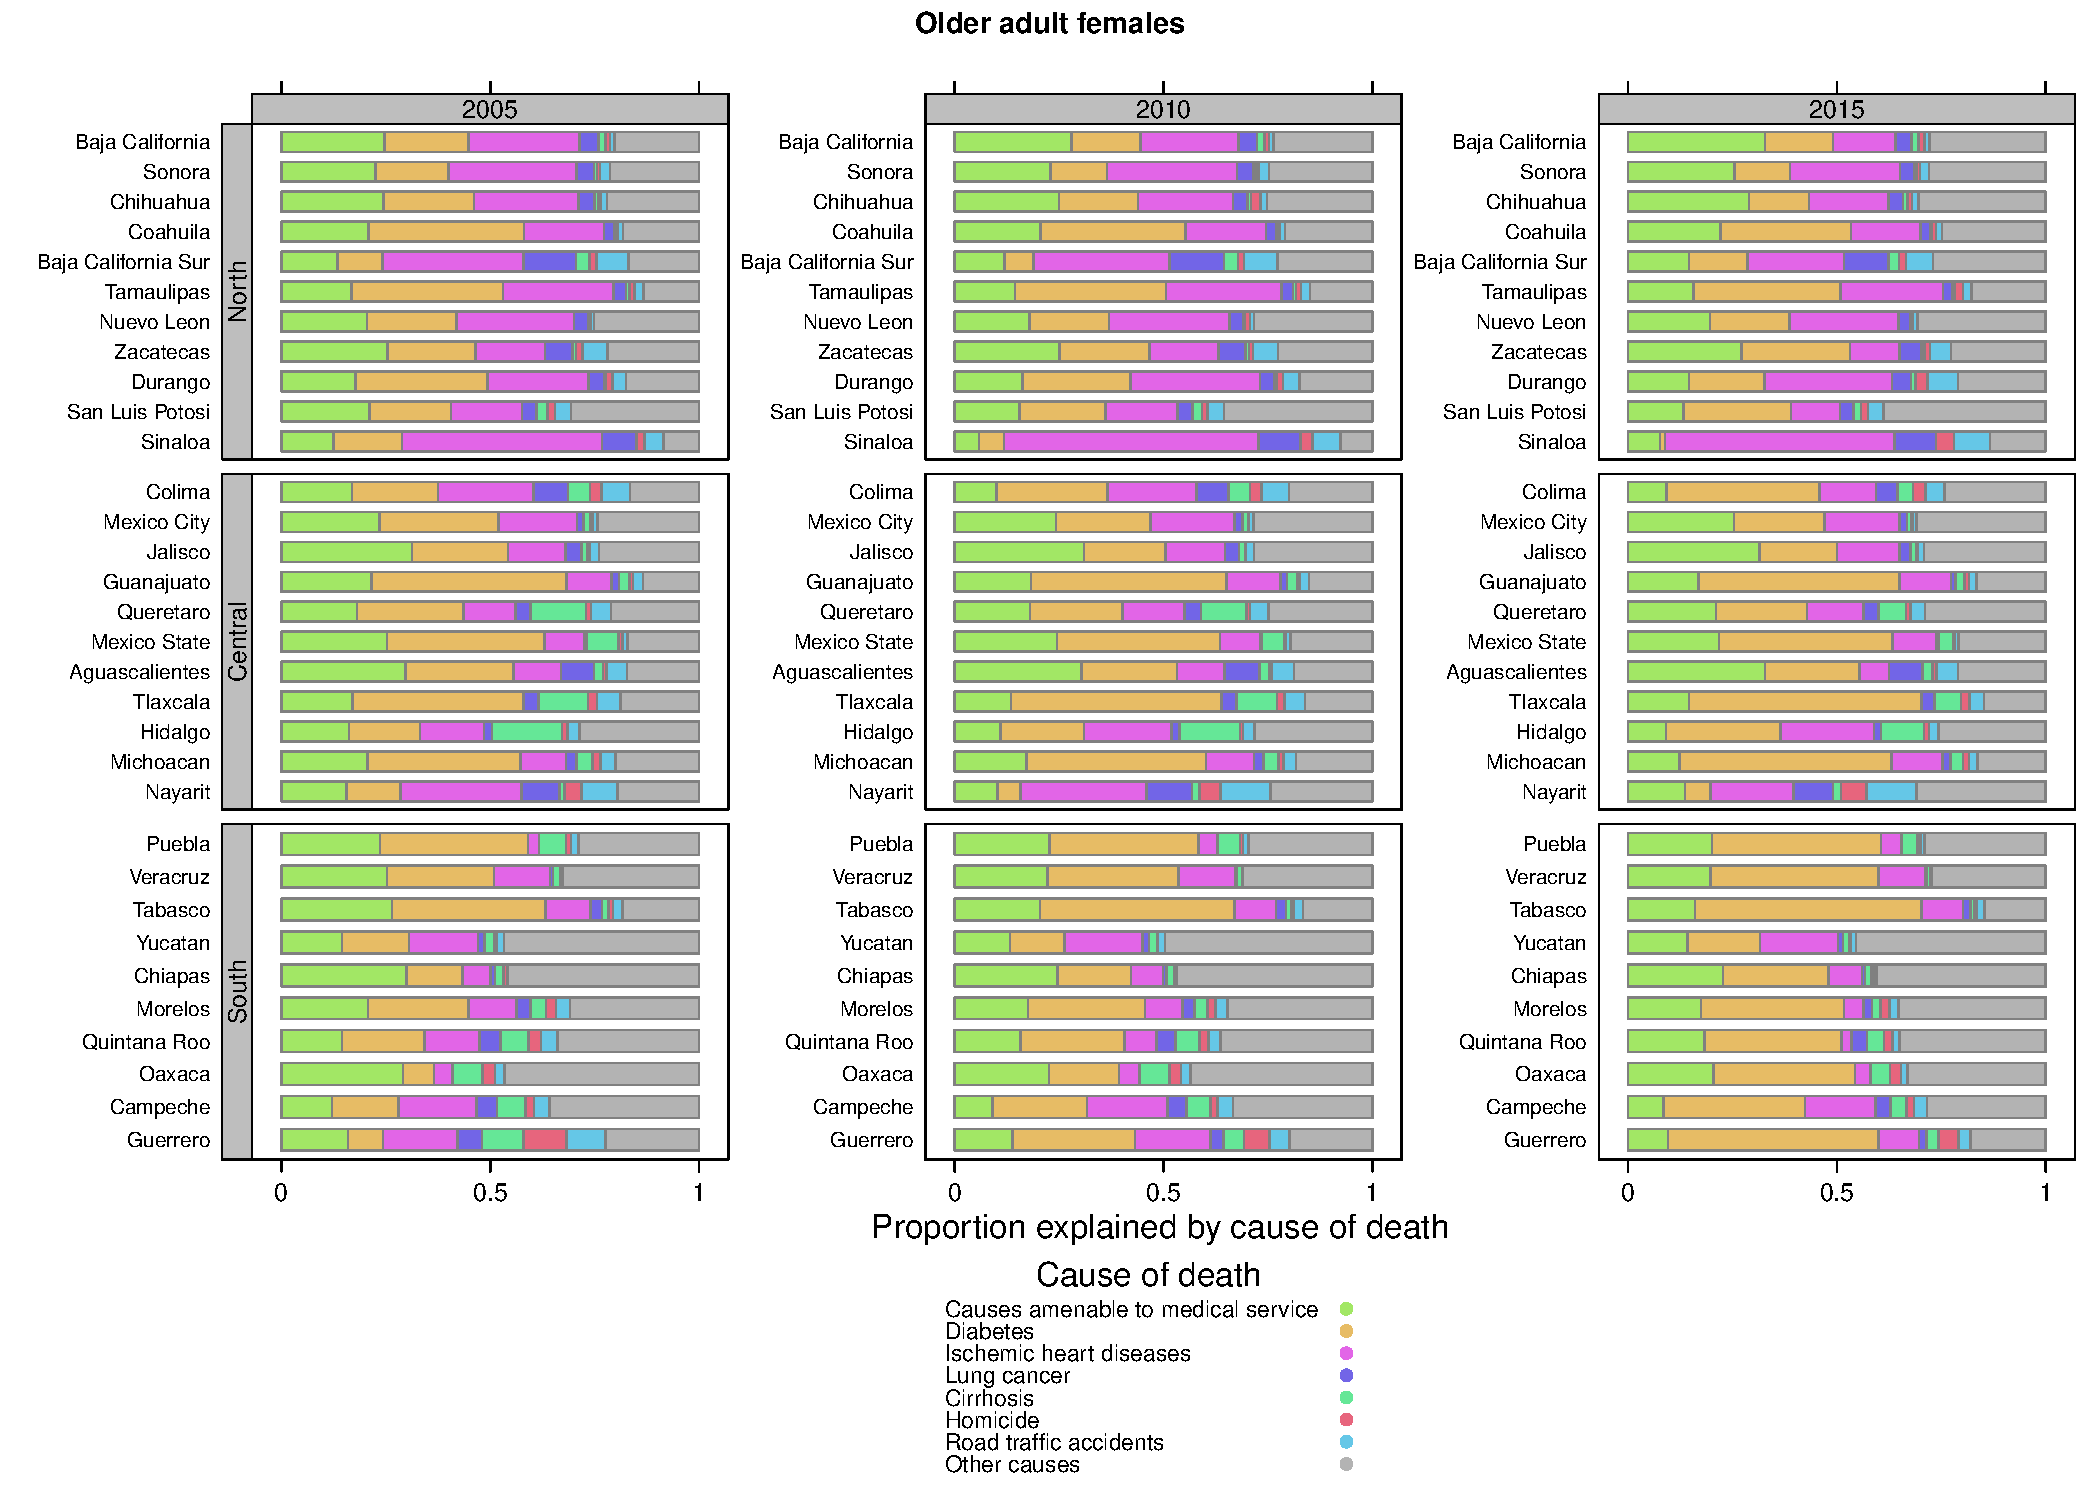
\includegraphics[scale=.5]{Figures/Figure_prop_oaf.pdf}
\end{center}
\end{figure}


%\begin{figure}
%\centering
%\caption{Suicide contribution to the gap with benchmark by age group for %males Source: own calculations.}
%\begin{center}
%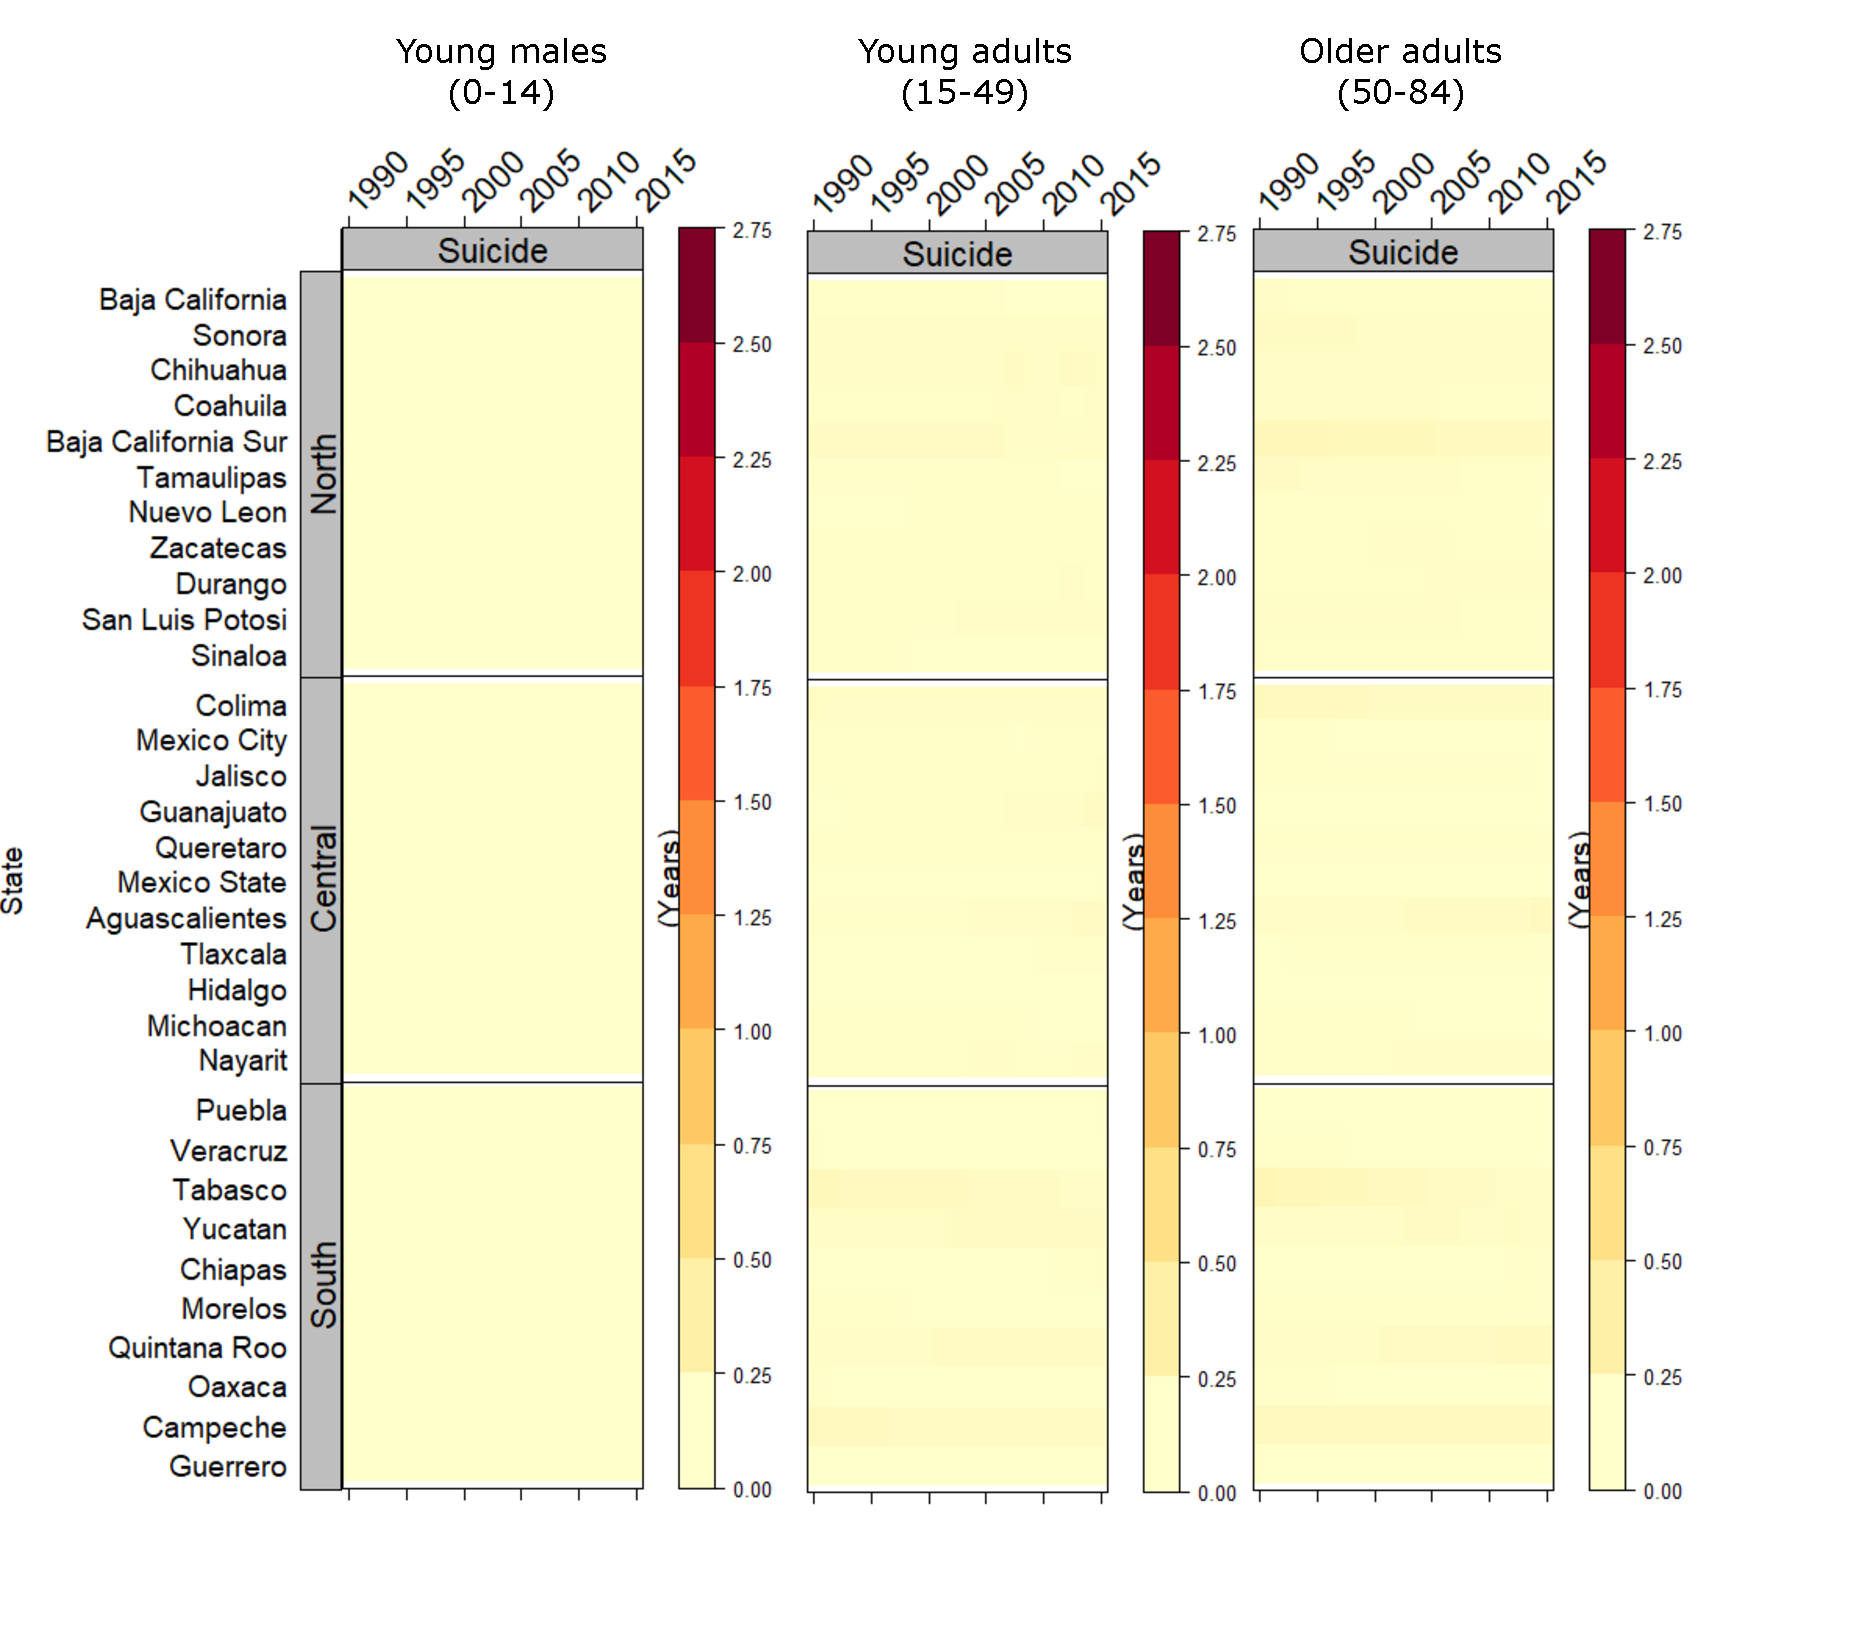
\includegraphics[scale=.5]{Figures/Suicide_Appendix.pdf}
%\end{center}
%\end{figure}



\bibliography{AburtoRiffe_Bib}







\end{document}
